\documentclass[a4paper,11pt,oneside,openany]{jsbook}
\usepackage{graphicx,enumerate}
\usepackage{algorithm}
\usepackage{algorithmic}
\usepackage{float}
\usepackage{amssymb}
\usepackage{mathabx}
\usepackage{longtable}
\usepackage{supertabular}
\usepackage{subfigure}
\usepackage{lscape}

\pagestyle{plain}
\setlength{\textwidth}{\fullwidth}
\setlength{\evensidemargin}{\oddsidemargin}
\def\vector#1{\mbox{\boldmath $#1$}}
\begin{document}
\thispagestyle{empty}
%------------------------------標題紙作成エリア----------------------------%
2015年度 卒業論文%1
\bigskip%2
\LARGE%3
\begin{center}
卒業論文
\end{center}
\bigskip\bigskip\bigskip\bigskip\bigskip\bigskip\bigskip %7
\begin{center} %8
Differential EvolutionにおけるArchiveの性能評価及び改善
\end{center}
\large %11
\begin{center}
Evaluating And Improvement Of Performance Of Archive In Differential Evolution
\end{center}
\bigskip\bigskip\bigskip\bigskip\bigskip\bigskip\bigskip\bigskip\bigskip\bigskip
\bigskip\bigskip\bigskip\bigskip\bigskip\bigskip\bigskip\bigskip\bigskip
\Large %17
\begin{center}
教養学部学際科学科 総合情報学コース
\end{center}
\Large %17
\begin{center}
指導教員: 福永 アレックス
\end{center}
\LARGE %21
\begin{center}
山村 武史
\end{center}
\normalsize
%---------------------------------目次エリア-------------------------------%
\thispagestyle{empty}
\tableofcontents
%---------------------------------本文エリア-------------------------------%

\chapter{序論}
\section{研究の背景}
実数値最適化問題とは,ある$D$次元の実数値ベクトル$\vector{x} = (x_1, x_2, ..., x_D)$と,それを評価する関数$f(\vector{x})$が与えられた時に,その評価関数を最小もしくは最大化するような実数値ベクトル$\vector{x}$を求める問題である.
対象問題が,局所解を複数持つ多峰性を有する場合,局所解を避け,大域的な最適解を求めることが実数値最適化問題において重要な課題の一つである.また多くの実問題については,対象問題が単峰性か,多峰性か,及び変数分離可か不可かなどといった情報を探索の事前に知ることは困難である.このような$\vector{x}$の目的関数値$f(\vector{x})$しか利用出来ない実数値最適化問題をblack-box optimizationと呼ぶ.
そのような実数値最適化問題を対象とする確率的手法の一つとして,差分進化(Differential Evlolution:DE) \cite{Storn} が用いられる.DEはEvolutionary Algorithm(EA)のひとつであり,EAとは,変化と選択に基づく世代交代により解が進化していく計算の総称である.
最初のDEは,1995年にStornとPriceらによって提案された.
DEは単純なアルゴリズムでありながら,他の探索手法と比べても良好な性能を有することが報告されている
 \cite{Storn} \cite{ExDE} .
このためDEは実問題への多くの適用例が報告されている \cite{ExDE} .

\section{関連研究}
DEの探索性能は用いる制御パラメタに大きく依存し,そのパラメタは集団数,スケール係数$F$,交叉率$CR$である.しかしこれらのパラメタの適切な値は使用する関数や問題設定によって異なり,実問題を解く上でこれらのパラメタをユーザーが試行錯誤する必要がある.
これらのパラメタを探索中に適応的に変化させていく適応型のDEに関する研究が数多く行われている.
それら適応型のDE手法としてはJADE \cite{JADE} ,SHADE \cite{SHADE} などが挙げられる.
JADEでは適応戦略以外に,探索性能を強化するために過去の劣解を保持するアーカイブを使用する.
変異ベクトル作成時にアーカイブに保存された劣解を用いることで,解集団における多様性の維持に役立つ.

しかしアーカイブは問題設定などによっては,探索性能の向上にうまくつながらないこともある \cite{JADE} .JADEにてその性能比較を行った先行研究では,次元数が高い時にアーカイブは解集団の探索性能を向上させた.一方で,次元数に対して十分な集団数をもつ場合,アーカイブ使用時の方がJADEにおいてその探索性能は低下した.これは,次元数や集団数によって,解集団が多様性を維持出来ない場合に,アーカイブがその多様性を向上させるためと述べられている.しかしながらアーカイブが解集団にどの程度多様性を与えているのか,そもそも多様性とは何か,なんらかの尺度による調査はなされていない.
本論文では,アーカイブを使用することで解集団における多様性を確かに維持できているのか,次元数,集団数の違いが多様性維持にどのように影響を与えているのか解明するとともに,従来のアーカイブを改善した手法をいくつか提案する.

\section{本研究の目的}
本研究の目的は2つある.
\begin{enumerate}
\item アーカイブが多様性の維持にどのように役割をはたしているのか調査する
\vspace{3mm}
\newline
アーカイブには,生存選択の時に,劣解として,子個体に上書きされた親個体が保存される.変異ベクトル作成時にアーカイブに保存された劣解を用いることで,解集団における多様性の維持に役立つ.本研究では,アーカイブを使用することで,解集団における多様性を確かに維持できているのか,次元数,集団数の違いが多様性維持にどのように影響を与えているのか多様性評価指標$r_s$,$r_f$を基に調査する.
\newline


\item アーカイブを改良することで,探索性能を向上できないか新たな手法を提案する.
\vspace{3mm}
\newline
アーカイブは多くの適応DEについて使われているにも関わらず,そのシステムについての改良は他の制御パラメタであるスケール係数$F$や交叉率$CR$に比べ試みられていない.
アーカイブ性能の分析をふまえた上で,その改善をはかるための新たな手法を提案する.
\end{enumerate}


\section{本論文の構成}
本論文は以下の通りに構成される。2 章でDEの詳細と適応DE,アーカイブの使用例について説明する.3 章ではアーカイブの性能を多様性評価指標$r_s$,$r_f$の値をもとに調査する.4章ではアーカイブの改善を試みた二つの手法について説明する.5章では本研究における知見をまとめる.

\chapter{Differential Evolutionとアーカイブ}
\section{Differential Evolution}
まず基本的なDEアルゴリズムについて説明する.DEの集団中の各個体$i \in \{1, ..., N\}$は対象問題の解ベクトル$\vector{x}^i = (x^i_1, ..., x^i_D)$で表現される.ここで$N$は集団数,$D$は次元数である.探索開始時に各個体は探索領域内にランダムに初期化される.その後,突然変異戦略による変異個体の生成,交叉による子個体の生成,生存選択を,探索の終了条件を満たすまで繰り返す.

\begin{table}[h]
  \begin{center}
  \caption{DEにおける代表的な突然変異戦略}
    \begin{tabular}{ll} \hline
      突然変異戦略 & 定義  \\ \hline
      rand/1 & $\vector{v}^{i} := \vector{x}^{r1} + F\cdot(\vector{x}^{r2} - \vector{x}^{r3})$ \\
      rand/2 & $\vector{v}^{i} := \vector{x}^{r1} + F\cdot(\vector{x}^{r2} - \vector{x}^{r3}) + F\cdot(\vector{x}^{r4} - \vector{x}^{r5})$ \\
      best/1 & $\vector{v}^{i} := \vector{x}^{best} + F\cdot(\vector{x}^{r1} - \vector{x}^{r2})$ \\
      best/2 & $\vector{v}^{i} := \vector{x}^{best} + F\cdot(\vector{x}^{r1} - \vector{x}^{r2}) + F\cdot(\vector{x}^{r3} - \vector{x}^{r4})$ \\
      current-to-rand/1 & $\vector{v}^{i} := \vector{x}^{i} + F\cdot(\vector{x}^{r1} - \vector{x}^{i}) + F\cdot(\vector{x}^{r2} - \vector{x}^{r3})$ \\
      current-to-best/1 & $\vector{v}^{i} := \vector{x}^{i} + F\cdot(\vector{x}^{best} - \vector{x}^{i}) + F\cdot(\vector{x}^{r1} - \vector{x}^{r2})$ \\
      current-to-$p$best/1 & $\vector{v}^{i} := \vector{x}^{i} + F\cdot(\vector{x}^{pbest} - \vector{x}^{i}) + F\cdot(\vector{x}^{r1} - \vector{x}^{Ar2})$ \\
      rand-to-$p$best/1 & $\vector{v}^{i} := \vector{x}^{r1} + F\cdot(\vector{x}^{pbest} - \vector{x}^{r1}) + F\cdot(\vector{x}^{r2} - \vector{x}^{Ar3})$ \\ \hline
    \end{tabular}
  \end{center}
\end{table}


各世代$t$において各変異個体${\vector{v}^{i,t}}$となる変異ベクトルを集団中の複数の個体に突然変異戦略を適用することで生成する.代表的な突然変異戦略を表(2.1)にて示す.表(2.1)において,スケール係数${F\in(0,1]}$は突然変異の大きさを調整する制御パラメタである.$\vector{x}^{r1},\vector{x}^{r2},\vector{x}^{r3},\vector{x}^{r4},\vector{x}^{r5}$は${\vector{x}^i}$と互いと異なるように集団$\vector{P} = \{ \vector{x}^1, ..., \vector{x}^N \}$からランダムに選択した個体である.$\vector{x}^{best}$は各世代における最良個体であり,$\vector{x}^{pbest}$は集団ベクトルを目的関数値の良い順に並び替え,${p\in[0,1]}とした時の上位$max$(N \times p, 2)$個体からランダムに選択した個体である.
current-to-$p$best/1とrand-to-$p$best/1の際にoptinとしてアーカイブ戦略を取ることが先行研究において提案された \cite{JADE} .アーカイブ戦略を取る場合,${\vector{x}^{Ar2}}$,${\vector{x}^{Ar3}}$を集団ベクトルと後述のアーカイブベクトルの集合からランダムに選択する.アーカイブ戦略を取らない場合は,${\vector{x}^{Ar2}}$,${\vector{x}^{Ar3}}$を集団ベクトルからランダムに選択する.
それぞれの突然変異戦略において,best/1,best/2は変異個体{$\vector{v}^i$}を最良個体$\vector{x}^{best}$の付近に生成する.
それに対しcurrent-to-best/1は対象個体から$\vector{x}^{best}$にむかうように変異個体{$\vector{v}^i$}を生成する.そのためrand/1やrand/2などに比べ局所的探索能力が強い戦略である.また加える差ベクトルの数が多いほど多様な変異個体{$\vector{v}^i$}を生成しやすい.

次に親個体$\vector{x}_i$と変異個体$\vector{v}_i$を交叉させることで子個体$\vector{u}_i$を生成する.DEの代表的な交叉手法には二項交叉(binomial crossover)と指数交叉(exponential crossover)がある.以下では二項交叉について紹介する.二項交叉では交叉率$CR \in [0,1]$とランダムに選択した$j_{rand} \in \{1,...,D\}$に基づき,Algorithm 1のように子個体$\vector{u}^i = (u^i_1,...,u^i_D)$の各要素$u^i_j$を決定する.
DEのアルゴリズムの全体をAlgorithm 2 に示す.


\begin{algorithm}
\caption{二項交叉}
\label{alg:pbnf}
\begin{algorithmic}
\STATE $j_{rand} = \rm{randi}[1, D]$;
\FOR{$j=1$ to $D$}
  \IF {$\rm{rand}[0,1) \leqq $ \OR $j == j_{rand} $}
    \STATE $u^i_j$ := $v^i_j$;
  \ELSE
    \STATE $u^i_j$ := $x^i_j$;
  \ENDIF
\ENDFOR
\end{algorithmic}
\end{algorithm}


全ての個体が子個体を生成した後,次世代に残る個体を決定する.DEでは親個体と子個体の目的関数値を評価関数$f(\vector{x})$を用いて比較し,目的関数値の良いものを次世代へ残す.
この選択の際,current-to-$p$best/1,及びrand-to-$p$best/1のアーカイブ戦略を用いた場合,子個体より劣っていた親個体$\vector{x}^i$を,アーカイブに保存する.アーカイブのサイズは集団ベクトルのサイズと等しく,そのサイズを超えた場合ランダムに選択したアーカイブ中の個体を超過分だけ取り除く.


\newpage
\begin{algorithm}
\caption{Differential Evolution}
\label{alg:pbnf}
\begin{algorithmic}
\STATE 集団$P={\vector{x}^1,...,\vector{x}^N}$の初期化;
\WHILE {探索終了条件を満たしていない}
    \FOR{$i=1$ to $N$}
        \STATE 突然変異戦略を用いて変異個体{$\vector{v}^i$}を生成;
        \STATE $\vector{x}^i$と$\vector{v}^i$に交叉を適用し,子個体$\vector{u}^i$を生成;
    \ENDFOR
    \FOR{$i=1$ to $N$}
        \IF {$f(\vector{u}^i) \leqq f(\vector{x}^i)$}
            \STATE $\vector{x^i} \rightarrow {A}$;
            \STATE {$\vector{x}^i :=\vector{u}^i$};
        \ENDIF
    \ENDFOR
    \STATE もしアーカイブがアーカイブサイズ$|A|$を超えていれば,超えた分だけランダムに削除;
\ENDWHILE
\end{algorithmic}
\end{algorithm}
\newpage

\section{DEの探索における収束性と多様性}
通常のDEについて前節で説明をした.そしてDEの探索性能は一般的に収束性と多様性の間のバランスを左右するパラメタによって決まる.ここでDEにおける収束性と多様性について再考する.

収束性は,良好な解の近傍に新しい解を発生させることにより向上する.DEにおいては,ステップ幅を調整する$F$の値を小さくしたり,子ベクトルが変位ベクトルに近くなるように$CR$を大きくするなどが,収束性を向上させる.収束性の向上は最適解により早く近づくことに繋がる一方,局所解に陥りやすくなるという欠点がある.

多様性は,広い範囲で新しい解を発生させることにより向上する.DEにおいては.ステップ幅を調整するFの値を大きくしたり,急速な収束を差避けるため$CR$を小さくする,またアーカイブによる突然変異戦略をとるなどが挙げられる.これによって,大域的な最適解を発見出来る可能性は高くなる代わりに,収束性が低下してしまうという問題がある.

このように収束性と多様性は両者ともトレードオフの関係にあたり,収束性と多様性どちらを優先するかはその探索過程で適応的に変化させる必要がある.これを可能にするため,パラメタ$F$と$CR$を探索中に変化させる適応型のDEとしてJADE\cite{JADE}やSHADE\cite{SHADE}があげられる.次の節ではこれらの手法について,紹介する.

\section{Adaptive Differential Evolution (JADE)}
JADE \cite{JADE} はZhangらによって2009年に提唱された適応型DEの一つである.JADEではDEの探索性能を大きく左右するスケール係数$F$と交叉率$CR$を通常のDEのように固定するのではなく,探索中に自動調整する.その自動調整のために適応メタパラメタ$\mu _F,\mu _{CR}$ を使用する.これらのパラメタは探索開始時に0.5に初期化する.通常のDEでは$F$と$CR$は共通する変数であったが,JADEでは,集団の各個体\vector{x^i}ごとに適応パラメタ$F_i$,$CR_i$を持つ.
そして世代のはじめに$F_i$と$CR_i$を,$\mu _F,\mu _{CR}$をもとにそれぞれ式(2.1),式(2.2)のように更新する.

\begin{eqnarray}
  F_i & = & \rm{randc}(\mu _F, 0.1) \\
  CR_i & = & \rm{randn}(\mu _{CR}, 0.1)
\end{eqnarray}

ここで$\rm{randc}(\mu,\sigma)$は位置パラメタ$\mu$と尺度パラメタ$\sigma$のコーシー分布に従う乱数,$randn(\mu,\sigma^2)$ は平均$\mu$,標準偏差$\sigma^2$の正規分布に従う乱数である.$F_i$の値が$F_i>1$の場合は
$F_i=1$とし $F_i\leqq0$の場合は再び式2.1を用いて生成を行う.$CR_i$の値が区間より外の場合は超えた方の境界値で置き換えられる.
コーシー分布は正規分布に比べ,よりひろがりを持つ分布である.そのためコーシー乱数を使った場合の方が,正規乱数に比べ,多様性を維持したパラメタを生成することが出来る.
各世代の終了後に,成功した${F}$と${CR}$に基づき$\mu_F, \mu_{CR}$を更新する.これらの更新式は式(2.3),式(2.4)となる.

\begin{eqnarray}
  \mu_F & = & (1 - c)\cdot\mu_F + c\cdot mean_L(S_F)\\
  \mu_{CR} & = & (1 - c)\cdot\mu_{CR} + c\cdot mean_A(S_{CR})
\end{eqnarray}

ここで$S_F,S_{CR}$とは,各世代において,生存選択を行う際に親個体よりも優れた変異個体を生成することの出来た$F_i,CR_i$の集合である.次に$c\in[0,1]$は学習率であり推奨値は0.1である.学習率$c$が小さいほど,更新前の$\cdot\mu_F,\cdot\mu_{CR}$に近い値となり,学習率$c$が大きいほど,今の世代で成功した${F}$と${CR}$の値による影響が大きくなる.
また$\rm{mean}_A(\cdot)$は算術平均, $\rm{mean}_L(\cdot)$はLehmer平均でありそれぞれ式(2.5),式(2.6)となる.

\begin{eqnarray}
  mean_A(S) & = \frac{1}{|S|}\sum_{s\in S}s \\
  mean_L(S) & = \frac{\sum_{s\in S}s^2}{\sum_{s\in S}s}
\end{eqnarray}
ここで$S=(s_1,..., s_{|S|})$は$S_F,S_CR$のいずれかである.
JADEのパラメタ適応のメカニズムは,探索中に優れた解を生み出すことの出来たスケーリング係数$F$,交叉率$CR$に近づく形で,それらのパラメタを更新していく.
そのため,理想的なスケーリング係数$F$,交叉率$CR$が,問題設定や探索途中で変わっていくDEにおいて,適切なパラメタを選択することがJADEにおいて可能である.
JADEのアルゴリズムの全体をAlgorithm 3 に示す.
\newpage
\begin{algorithm}
\caption{JADE}
\label{alg:pbnf}
\begin{algorithmic}
\STATE 集団$P={\vector{x}^1,...,\vector{x}^N}$の初期化;
\STATE  $\mu_F := 0.5; \mu_{CR} := 0.5f$で初期化;
\WHILE {探索終了条件を満たしていない}
    \STATE $S_F := \emptyset, S_{CR} := \emptyset$;
    \FOR{$i=1$ to $N$}
        \STATE $F_i := \rm{randc}(\mu _F, 0.1)$ \\
        \STATE $CR_i := \rm{randn}(\mu _{CR}, 0.1)$ \\
        \STATE 突然変異戦略を用いて変異個体{$\vector{v}^i$}を生成;
        \STATE $\vector{x}^i$と$\vector{v}^i$に交叉を適用し,子個体$\vector{u}^i$を生成;
    \ENDFOR
    \FOR{$i=1$ to $N$}
        \IF {$f(\vector{u}^i) \leqq f(\vector{x}^i)$}
            \STATE $\vector{x^i} \rightarrow {A}$;
            \STATE {$\vector{x}^i:=\vector{u}^i$};
            \STATE $S_F := {F_i}, S_CR := {CR_i};$
        \ENDIF
    \ENDFOR
    \IF {$ S_F,S_{CR} \neq \emptyset$}
        \STATE $\mu_F := (1 - c)\cdot\mu _F + c\cdot \rm{mean}_L(S_F)$
        \STATE $\mu_{CR} := (1 - c)\cdot\mu _{CR} + c\cdot  \rm{mean}_A(S_{CR})$
    \ENDIF
    \STATE もしアーカイブがアーカイブサイズ$|A|$を超えていれば,超えた分だけランダムに削除;
\ENDWHILE
\end{algorithmic}
\end{algorithm}
\newpage

\section{Succes-History based Adaptive Differential Evolution (SHADE)}
前述のJADEにつづいて本項では過去の成功したパラメタをもとに適応的にFとCRを変化させるSHADEを紹介する.
JADEでは各世代ごとの成功した有望なパラメタ設定$S_{CR}$, $S_{F}$に近づくようにパラメタを適応させていった.これは$S_{CR}$,$S_F$が対象問題に適したパラメタ値であることを前提としているが,不適切なパラメタ値が$S_{CR}$,$S_F$に含まれる可能性がある.これを防ぐため,SHADEでは大きさ$H$の履歴メモリ$M_F$,$M_{CR}$を用いてパラメタ適応を行う.これによってJADEに比べ多様なパラメタ値を保持しながら探索を行えるため,よりロバストな探索が可能となる.
ここで,離散メモリは,$M_F = (M_{F,1},...,M_{F,H})$,$M_{CR}= (M_{CR,1},...,M_{CR,H})$であり,すべての要素は探索開始時に0.5に初期化されている.JADEと同様に集団の各個体\vector{x^i}ごとに適応パラメタ$F_i$,$CR_i$を持ち,これらのパラメータを
各世代のはじめに$[1,H]$の範囲からランダムに選択したメモリの添字$r$の要素$M_{F,r},M_{CR,r}$を用いて式(2.7),式(2.8)のようにして生成する.

\begin{eqnarray}
  F_i & = & \rm{randc}(M_{F,r}, 0.1) \\
  CR_i & = & \rm{randn}(M_{CR,r}, 0.1)
\end{eqnarray}

$F_i$の値が$F_i>1$の場合は$F_i = 1$とし $F_i\leqq1の$の場合は再び式2.7を用いて生成を行う.$CR_i$の値が[0,1]区間より外の場合は超えた方の境界値で置き換えられる.各世代の終了時に成功した$F_i,CR_i$の集合$S_F,S_{CR}$のLehmer平均を用いて,式(2.9),式(2.9)のようにメモリ$M_F,M_CR$を更新する.

\begin{eqnarray}
  M_{F,k} & = & mean_L(S_F)\\
  M_{CR,k} & = & mean_L(S_{CR})
\end{eqnarray}

ここで,$k \in [1,H]$は更新するメモリの要素を決定するパラメタであり,探索開始時に1に初期化され,以降更新を行うたびに1づつ増加していく.また,$k > H$となった場合は$k = 1$とする.探索が経過するに伴い$M_F,M_{CR}$には対象問題に適したかつ,多様なパラメタ設定が保持される.
一つのパラメタ$\mu _F, \mu _{CR}$で管理していたJADEに対し,$M_F = (M_{F,1},...,M_{F,H})$,$M_{CR}= (M_{CR,1},...,M_{CR,H})$とSHADEでは複数のパラメタを持つため,パラメタにおける多様性が維持しやすいのが特徴である.SHADEのアルゴリズムの全体をAlgorithm 4 に示す.

\newpage
\begin{algorithm}
\caption{SHADE}
\label{alg:pbnf}
\begin{algorithmic}
\STATE 集団$P={\vector{x}^1,...,\vector{x}^N}$の初期化;
\STATE $M _F$及び$M _{CR}$を0.5に初期化;
\STATE k = 1;
\WHILE {探索終了条件を満たしていない}
    \STATE $S_F := \emptyset, S_{CR} := \emptyset$;
    \FOR{$i=1$ to $N$}
        \STATE $r := \rm{randi}[1,H]$
        \STATE $F_i := \rm{randc}(M_F, 0.1)$ \\
        \STATE $CR_i := \rm{randn}(M_{CR}, 0.1)$ \\
        \STATE 突然変異戦略を用いて変異個体{$\vector{v}^i$}を生成;
        \STATE $\vector{x}^i$と$\vector{v}^i$に交叉を適用し,子個体$\vector{u}^i$を生成;
     \ENDFOR
    \FOR{$i=1$ to $N$}
        \IF {$f(\vector{u}^i) \leqq f(\vector{x}^i)$}
            \STATE $\vector{x^i} \rightarrow {A}$;
            \STATE {$\vector{x}^i := \vector{u}^i$};
            \STATE $S_F := {F_i}, S_CR := {CR_i};$
        \ENDIF
    \ENDFOR
    \IF {$ S_F,S_{CR} \neq \emptyset$}
        \STATE $M_{F,k}  :=  mean_L(S_F)$;
        \STATE $M_{CR,k}  :=  mean_L(S_{CR})$;
        \STATE $k = (k+1) \% H$;
    \ENDIF
    \STATE もしアーカイブがアーカイブサイズ$|A|$を超えていれば,超えた分だけランダムに削除;
\ENDWHILE
\end{algorithmic}
\end{algorithm}
\newpage
% \section{DEの探索における収束性と多様性}
% 通常のDE及び適応DEについて前節までで説明をした.そしてDEの探索性能は一般的に収束性と多様性の間のバランスを左右するパラメタによって決まる.ここでDEにおける収束性と多様性について再考する.

% 収束性は,良好な解の近傍に新しい解を発生させることにより向上する.DEにおいては,ステップ幅を調整する$F$の値を小さくしたり,子ベクトルが変位ベクトルに近くなるように$CR$を大きくするなどが,収束性を向上させる.収束性の向上は最適解により早く近づくことに繋がる一方,局所解に陥りやすくなるという欠点がある.

% 多様性は,広い範囲で新しい解を発生させることにより向上する.DEにおいては.ステップ幅を調整するFの値を大きくしたり,急速な収束を差避けるため$CR$を小さくする,またアーカイブによる突然変異戦略をとるなどが挙げられる.これによって,大域的な最適解を発見出来る可能性は高くなる代わりに,収束性が低下してしまうという問題がある.

% このように収束性と多様性は両者ともトレードオフの関係にあたり,収束性と多様性どちらを優先するかはその探索過程で適応的に変化する必要がある.その収束性と多様性をコントロールするパラメタである$F$と$CR$を探索過程では適応的に変化させるのが前節でのべたJADEやSHADEであった.
% アーカイブを使用した先行研究において,アーカイブ使用時に,使用しない時に比べて,常に性能を上げるのではなく,問題設定によっては探索性能が下がることがあった.これは多様性を向上させるアーカイブ戦略が,解探索における,収束性を下げることにつながるからである.

% 次章からは$F$や$CR$のように多様性維持に関わるアーカイブについても,適応的に変化させることでより良い結果が出るようになるのではないか.そもそもアーカイブが多様性の維持に対してどれほど有意な役割をもっているか解析を行う.

% \section{}
% アーカイブを使用した先行研究においてJADEの探索性能では少なくとも次元数に依存するという結果があった \cite{JADE} .JADEの探索性能は,次元数$D=30$,集団数$P=400$の時は,アーカイブ無しの時が良い探索性能を示したのに対し,
% 次元数$D=100$,集団数$P=400$の時は,アーカイブありの時の方が良い探索性能をしめした.これは次元数$D=100$に対して,集団数$P=400$が十分でなかったため,DE/NAでは多様性を十分維持出来なかった.
% そのためアーカイブが多様性維持に対して,大きな影響を与え,探索性能が,高次元,集団数が小さい場合JADEにおいて探索性能があがったと,先行研究では考察されている.
% 以下本論文ではアーカイブありのDEをDE/A,アーカイブなしのDEをDE/NAと定義する
% 本章では,そもそもアーカイブが解集団に多様性を維持させる機能が適応DEではなく通常のDEにおいてもあるか,調査する.





\chapter{アーカイブの解析}
\section{本章の目的}
アーカイブを使用した先行研究においてJADEの探索性能では少なくとも次元数に依存し,高次元のときに多様性維持に影響を与えるという結果があった \cite{JADE} .
本章ではそもそも解集団における多様性とは何か,2つの尺度で定義しなおし,アーカイブを使用することで,解集団における多様性を確かに維持できているのか,次元数,集団数の違いが多様性維持に影響を与えているのかどうかを調査する.これにより,アーカイブがどのような条件下で多様性維持に貢献するのかを明確にし,今後アーカイブを用いた優れたDEアルゴリズムを設計するために有益な知見を得る.

\section{実験設定}
解集団における多様性とはそもそも何か.本実験では次の2つの状態を多様な解を集団ベクトルが維持出来ていると捉えることにした.一つ目は解集団のベクトル同士が離れた位置にある状態であり,二つ目は解集団のベクトルの示す目的関数値のばらつきが大きい状態である.
これら二つの状態を図る指標としてそれぞれ多様性評価指標$r_s$, $r_f$を式(3.1),式(3.2)のように定義した.

\begin{eqnarray}
r_{s} = \sqrt{\frac{1}{P}\sum_{i=1}^{P} (d_i - d_{mean})^2} \\
r_{f} = \sqrt{\frac{1}{P}\sum_{i=1}^{P} (f(\vector{x}^i) - f_{mean})^2}
\end{eqnarray}

ここで$r_s$は集団ベクトルにおける重心からの距離の標準偏差,$r_f$は集団ベクトルにおける目的関数値$f(\vector{x})$の標準偏差である.また$P$は集団数,$D$は次元数である.$d_{mean}$,$f_{mean}$はそれぞれ集団ベクトルの重心からの距離の平均,集団ベクトルの目的関数値$f(\vector{x})$の平均であり式(3.3),式(3.4)で定義される.

\begin{eqnarray}
d_{mean} = \frac{1}{P}\sum_{i=1}^{P}d_i \\
f_{mean} = \frac{1}{P}\sum_{i=1}^{P}f(\vector{x}^i)
\end{eqnarray}

また集団ベクトルの重心からの距離$d_k$は式(3.5)のように定義される.ただし$k$は$k \in \{1, ..., P\}$となる整数値である.ここで$\vector{c}$は解集団$\vector{P} = \{ \vector{x}^{1}, ..., \vector{x}^{P} \}$における重心ベクトルであり,その要素を$\vector{c} = \{ \vector{c}_{1}, ..., \vector{c}_{P} \}$と表す.

\begin{eqnarray}
d_{k} = \sqrt{\sum_{i=1}^{D} (c_i - x_{k,i})^2}
\end{eqnarray}

解集団における重心からの距離の標準偏差と,目的関数値$f(\vector{x})$の標準偏差をしめすこれらの多様性評価指標$r_s$, $r_f$が大きければ解集団が多様性を維持出来ている事を示す.
また実験では目的関数として,Sphere関数(3.6),Rastrigin関数(3.7),Griewank関数(3.8)を使用した.Sphere関数は単峰性の関数であるのに対し,Rastrigin関数,及びGriewank関数は多峰性の関数である.Sphere関数及び,Rastrign関数は,設計変数間に依存関係がないのに対し,Griewank関数は設計変数間に依存関係を有する.

\begin{eqnarray}
  f_{Sphere}(\vector{x}) = \sum_{i=1}^D x_i^2
\end{eqnarray}

\begin{eqnarray}
f_{Rastrigin}(\vector{x}) &=& 10\cdot D+\sum_{i=1}^{D}\bigl( x_i^2-10\cos( 2\pi x_i) \bigr) \label{rastrigin}
\end{eqnarray}

\begin{eqnarray} f_{Griewank}(\vector{x}) & = & 1+\sum_{i=1}^{D}\frac{x_i^2}{4000}-\prod_{i=1}^{D} \Bigl(\cos
\bigl(\frac{x_i}{\sqrt{i}} \bigr) \Bigr) \label{griewank}
\end{eqnarray}

また実行可能領域は$[-100, 100]^D$であり,次元数$D$は$2,10,30,50,100$とした.また,集団数$P$は$10,30,50$とした.最大評価回数は1試行あたり$10,000 \times D$とし,試行回数は51回とした.使用したDEは突然変異戦略を式(3.2)のcurrent-to-$p$-bestとし,$F=0.5$,$CR=0.5$と,アーカイブを使用する時と使用しない場合で比較した.
また以下本論文ではアーカイブを使用した際のDEをDE/A,使用しなかった際のDEをDE/NAと表現する.ここでいうDE/Aとは式(3.9)における突然変異戦略current-to-$p$-bestにおいて$\vector{x}^{Ar2}$を集団PとアーカイブAの和集合から${\vector{x}^i}$と被らないようにランダムに選択したものである.DE/NAとは$\vector{x}^{Ar2}$を$\vector{x}_{i}$と被らないように集団ベクトルから選択したものである.

\begin{eqnarray}
\vector{v}^{i} = \vector{x}^{i} + F\cdot(\vector{x}^{pbest} - \vector{x}^{i}) + F\cdot(\vector{x}^{r1} - \vector{x}^{Ar2})
\end{eqnarray}



% 各世代ごとの重心からの距離の標準偏差について,51回の試行の平均値をのせたのが下記一覧である.
% 表?では目的関数値$f(x)$を用いて,多様性を計測した.ある世代tの解集団$P = {\vector{x}^{t,1}, ..., \vector{x}^{t,N}}$の $\vector{x}^{t,k}$を評価関数であるSphere関数で評価した値$f(s_{t,k})$の標準偏差について,51回の試行の平均値を載せたのが以下の図である.

\section{実験結果}
本節では,多様性評価指標$r_s$, $r_f$の推移を,次元数$D$,集団数$P$,複数の軸をもとに得られた実験結果について述べる.

まず次元数を軸に述べる.
次元数$D$が2である時の多様性評価指標$r_s$,$r_f$に着目すると,探索が200世代あたりで終了しているため,DE/AとDE/NA同士を比較すると$P\in\{10,30,50\}$の殆どの設定において差が見られない.
次元数$D$が10である時に着目すると,多様性評価指標$r_s$,$r_f$は両者とも集団数$P$が10のときのみ,DE/Aの方が,DE/NAと比較して多様性評価指標$r_s$,$r_f$を高く維持したまま,世代数が大きくなるに伴いその差を広げていった.それに対し集団数$P$が30,50である時DE/A,DE/NA同士でほとんど差が見られなかった.
次元数$D$が30の時に着目すると,集団数$P$が30の時でも,DE/AとDE/NAでの差が大きく広がっていることが分かる.
次元数$D$が50の時に着目すると,次元数$D$が30の時とほとんど変わらない.しかし注目すべき点は
集団数$P$が30である時,次元数$D$が30であった時と比較して,DE/AとDE/NAの同士の差の広がりが小さくなっている点である.これは多様性評価指標$r_s$,$r_f$の両方をみても同じ傾向が見られる.
次元数$D$が100の時を見ると,集団数$P$が10,30,50と全ての値を取る時で,DE/AとDE/NAの差の広がりが大きく見られた.

次に集団数を軸に述べる.
集団数$P$が10である時の多様性評価指標$r_s$,$r_f$に着目すると,次元数$D$が2の時はDE/A,DE/NAと比較して,ほとんど変わらなかったが,次元数$D$が10,30,50,100の時では大きくその差が開いた.しかしながら,その差の開きに着目すると,ほぼ同程度であった.
集団数$P$が30である時に着目すると,次元数$D$が2,10,30と高くなるに伴いDE/A,DE/NA同士でその差の開きは大きくなっていったが次元数$D$が30,50,100と高くなっても,差の開きは同程度のものであった.
集団数$P$が50である時に着目すると,次元数$D$が2,10,30,50,100と高くなるに伴い,DE/AとDE/NAの差の広がりが大きく見られた.


\section{考察}
実験結果から,集団数$P$が小さく,次元数$D$が高いほど,少なくともDEのSphere関数において,多様性評価指標$r_s$, $r_f$に基づき,アーカイブを使用することで解集団が多様性を維持したまま探索を行えていることがわかった.
これらのことからアーカイブが解集団の多様性維持に確かに貢献していること,集団数$P$,次元数$D$の設定によってアーカイブの性能が変わってくることが知見として得られた.
% これは,集団数$P$が少なく,次元数$D$が大きい時ほど,DEが解集団における多様性を維持したままた探索することが難しいことが原因と考えられる.そのためアーカイブによる多様性維持が探索に与える影響が大きく現れていると考えられる.

\newpage
\begin{figure}[htbp]
  \caption{横軸は評価回数の経過を1から2000世代目まで表示している.縦軸は51回試行した多様性評価指標$r_s$について,平均値を求めそれに対し,常用対数をとったものである.DE/AとDE/NAの二つのアルゴリズムを用いて,それぞれ次元数$D$を$2,10,30,50,100$とし,集団数$P$を$10,30,50$とした時の多様性評価指標$r_s$が推移する様子を示している.}
  \begin{center}
    \begin{tabular}{c}
      % 1
      \begin{minipage}{0.33\hsize}
        \begin{center}
          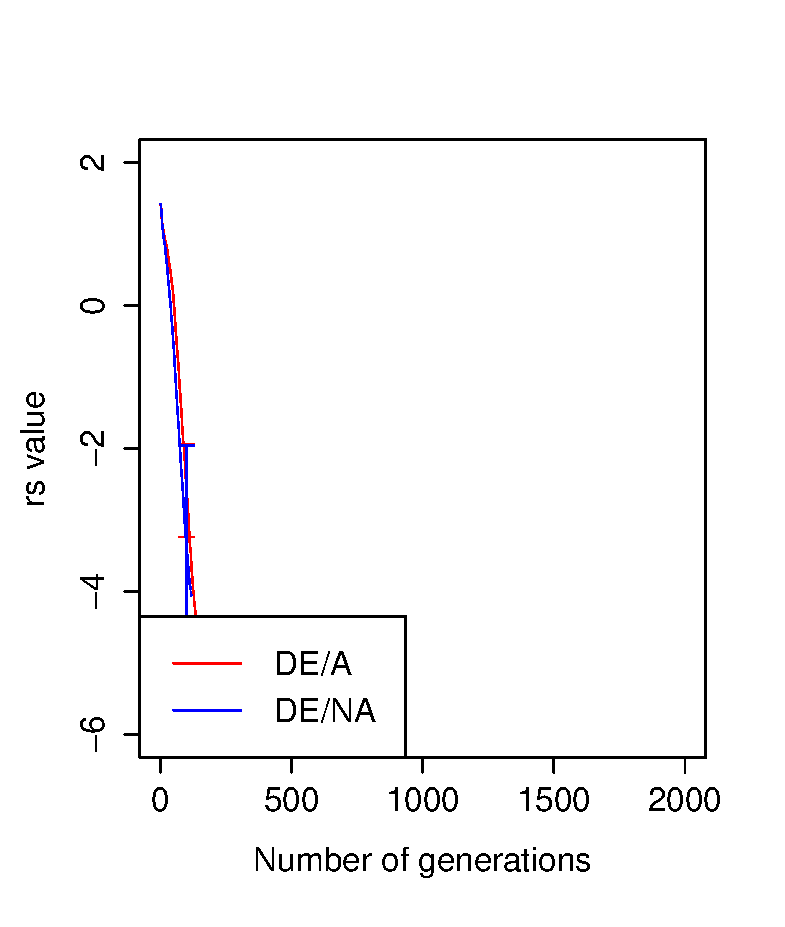
\includegraphics[clip, width=4.0cm]{P10D2.eps}
          \hspace{1.2cm}$P=10, D=2
 $       \end{center}
      \end{minipage}

      % 2
      \begin{minipage}{0.33\hsize}
        \begin{center}
          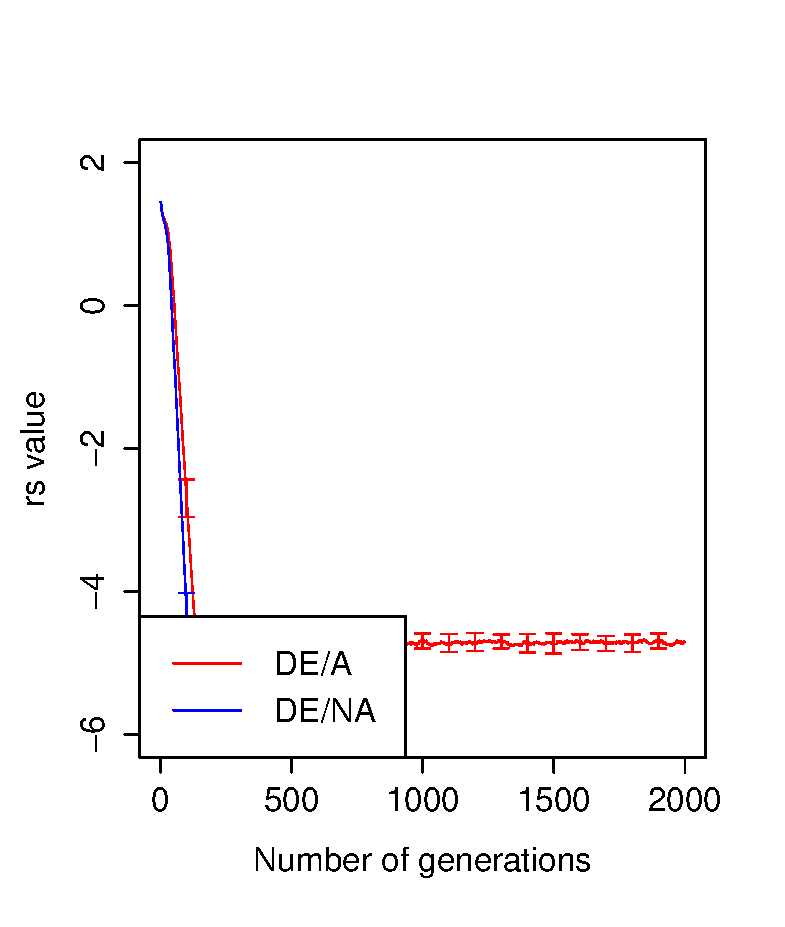
\includegraphics[clip, width=4.0cm]{P30D2.eps}
          \hspace{1.2cm}$P=30, D=2
 $       \end{center}
      \end{minipage}

      % 3
      \begin{minipage}{0.33\hsize}
        \begin{center}
          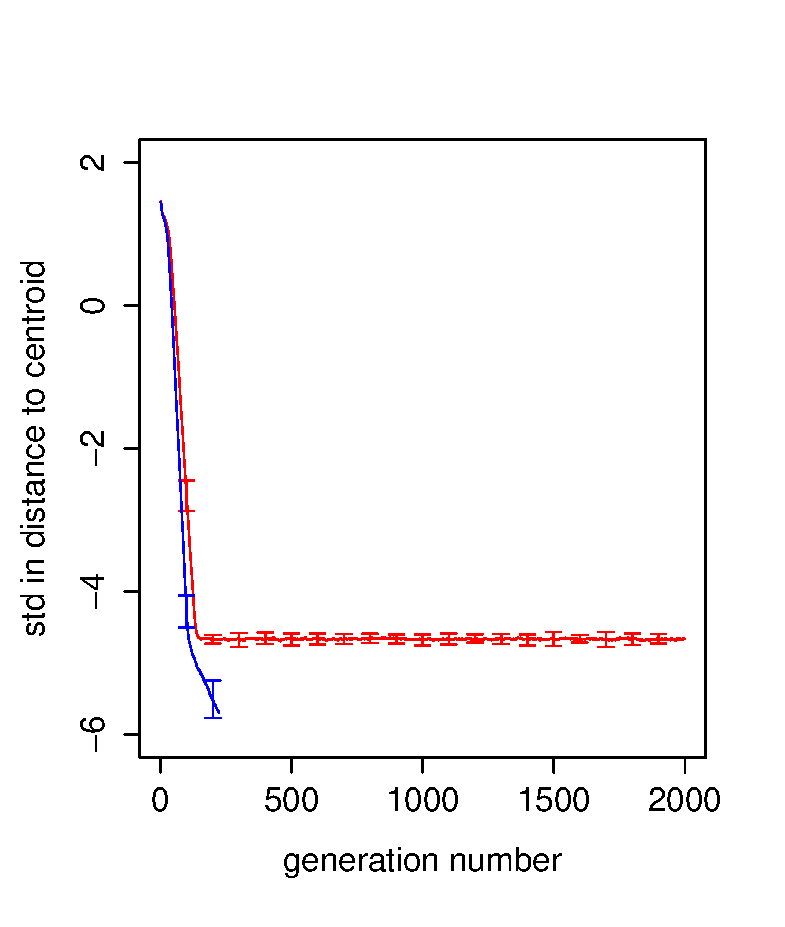
\includegraphics[clip, width=4.0cm]{P50D2.eps}
          \hspace{1.2cm}$P=50, D=2
 $       \end{center}
      \end{minipage}
    \end{tabular}
  \end{center}
\end{figure}
\begin{figure}[htbp]
  \begin{center}
    \begin{tabular}{c}


      % 1
      \begin{minipage}{0.33\hsize}
        \begin{center}
          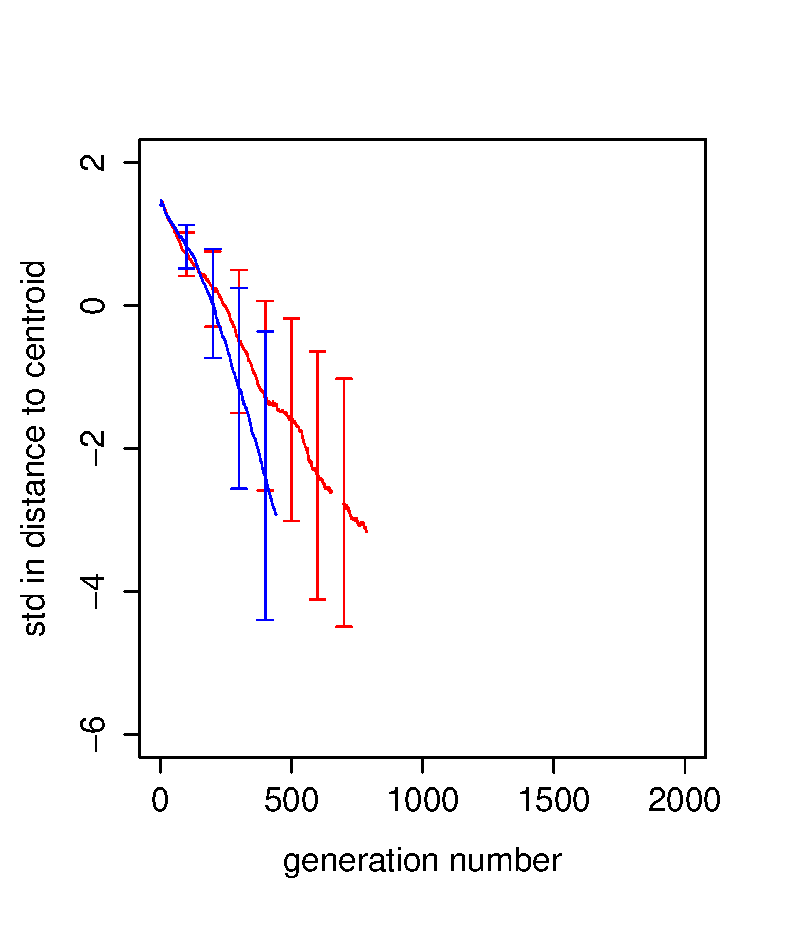
\includegraphics[clip, width=4.0cm]{P10D10.eps}
          \hspace{1.2cm}$P=10, D=10
$        \end{center}
      \end{minipage}

      % 2
      \begin{minipage}{0.33\hsize}
        \begin{center}
          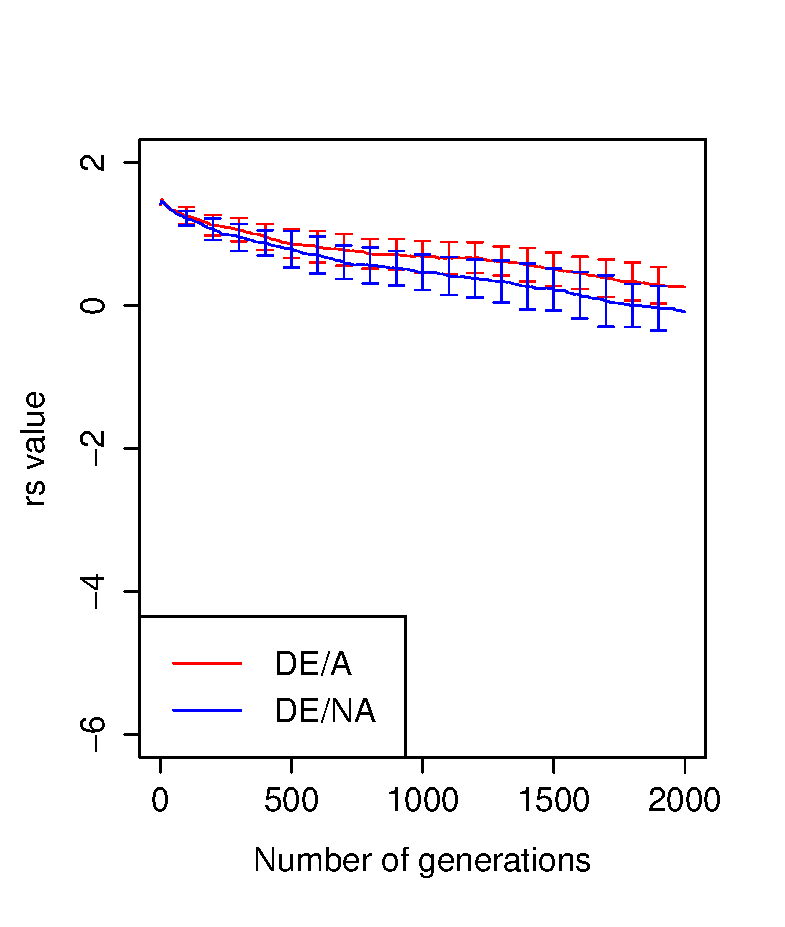
\includegraphics[clip, width=4.0cm]{P30D10.eps}
          \hspace{1.2cm}$P=30, D=10
$        \end{center}
      \end{minipage}

      % 3
      \begin{minipage}{0.33\hsize}
        \begin{center}
          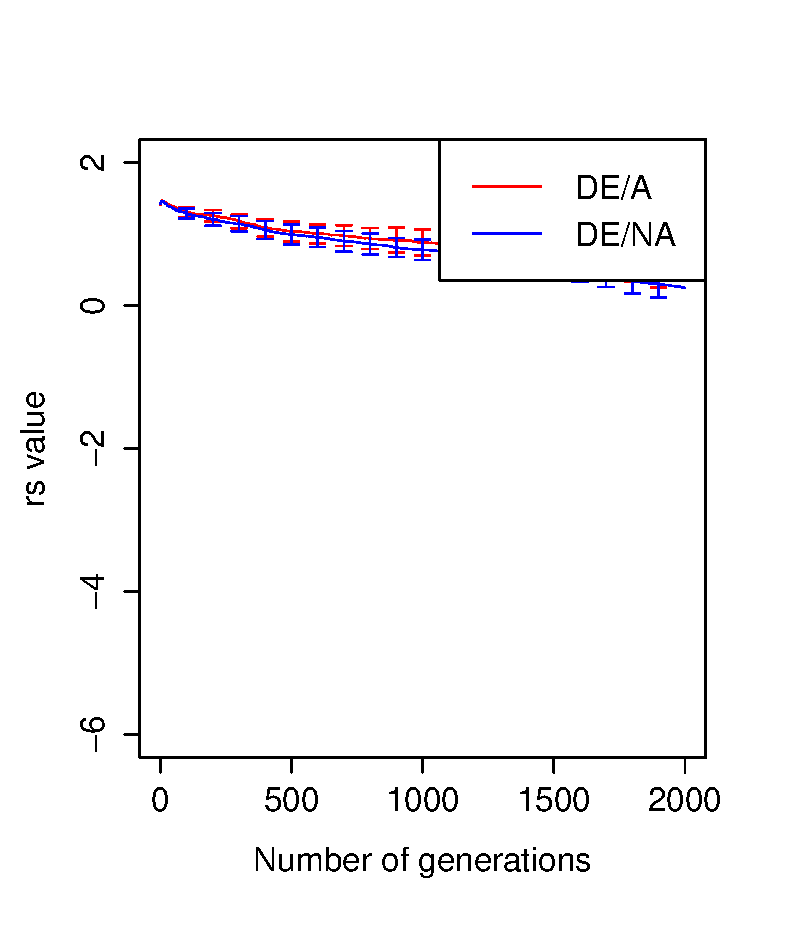
\includegraphics[clip, width=4.0cm]{P50D10.eps}
          \hspace{1.2cm}$P=50, D=10
$        \end{center}
      \end{minipage}
    \end{tabular}
  \end{center}
\end{figure}
\begin{figure}[htbp]
  \begin{center}
    \begin{tabular}{c}


      % 1
      \begin{minipage}{0.33\hsize}
        \begin{center}
          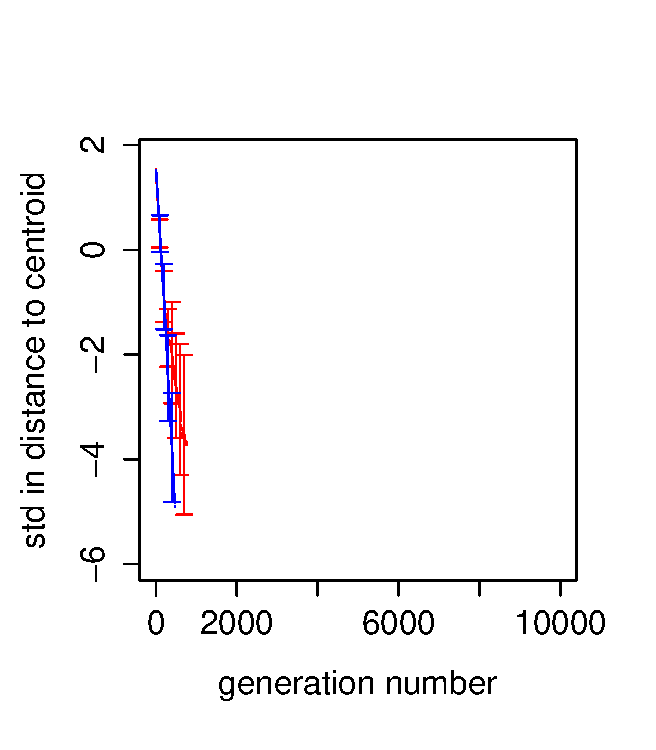
\includegraphics[clip, width=4.0cm]{P10D30.eps}
          \hspace{1.2cm}$P=10, D=30
$        \end{center}
      \end{minipage}

      % 2
      \begin{minipage}{0.33\hsize}
        \begin{center}
          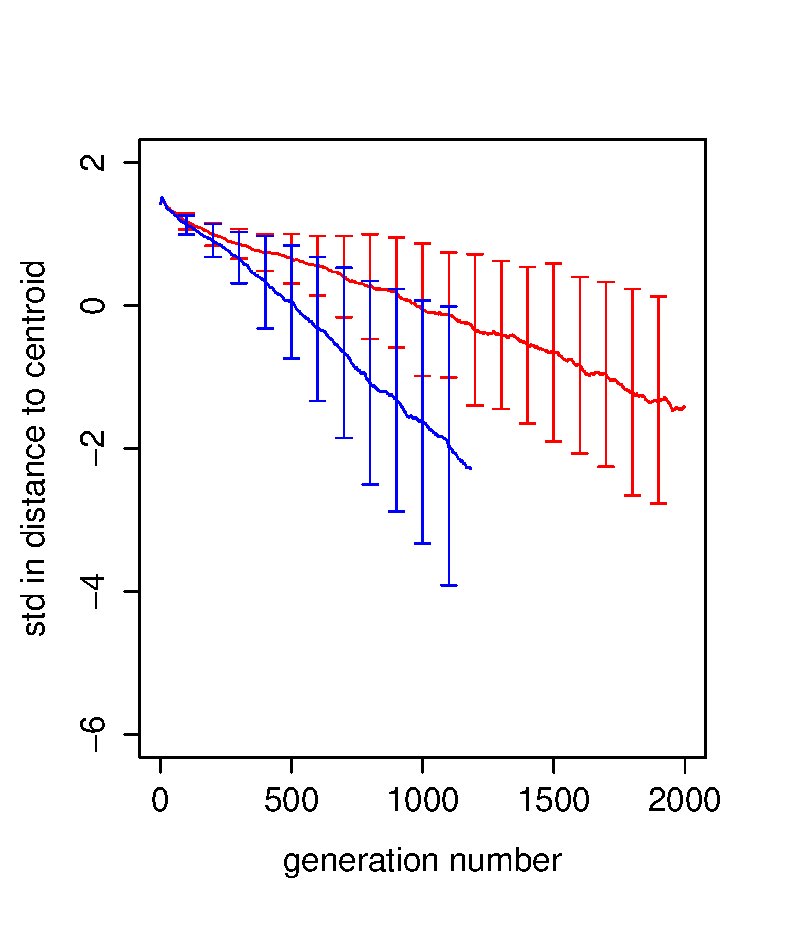
\includegraphics[clip, width=4.0cm]{P30D30.eps}
          \hspace{1.2cm}$P=30, D=30
$        \end{center}
      \end{minipage}

      % 3
      \begin{minipage}{0.33\hsize}
        \begin{center}
          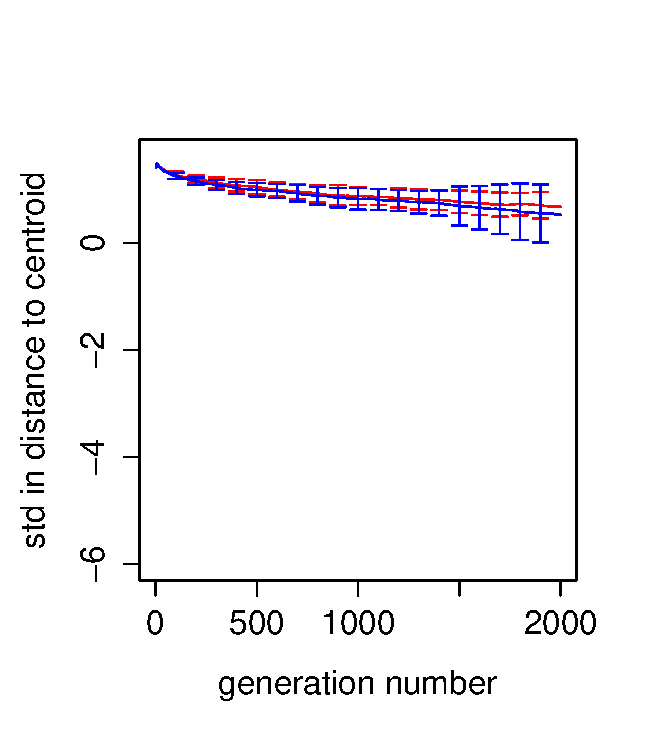
\includegraphics[clip, width=4.0cm]{P50D30.eps}
          \hspace{1.2cm}$P=50, D=30
$        \end{center}
      \end{minipage}
    \end{tabular}
  \end{center}
\end{figure}
\begin{figure}[htbp]
  \begin{center}
    \begin{tabular}{c}


      % 1
      \begin{minipage}{0.33\hsize}
        \begin{center}
          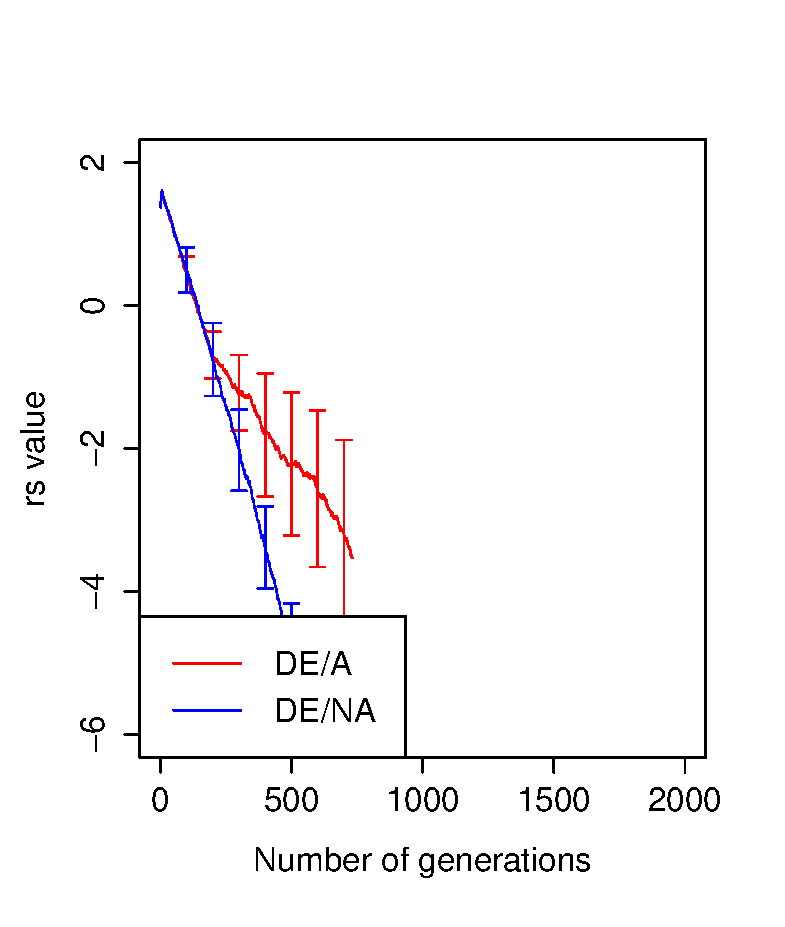
\includegraphics[clip, width=4.0cm]{P10D50.eps}
          \hspace{1.2cm} $P=10, D=50
$        \end{center}
      \end{minipage}

      % 2
      \begin{minipage}{0.33\hsize}
        \begin{center}
          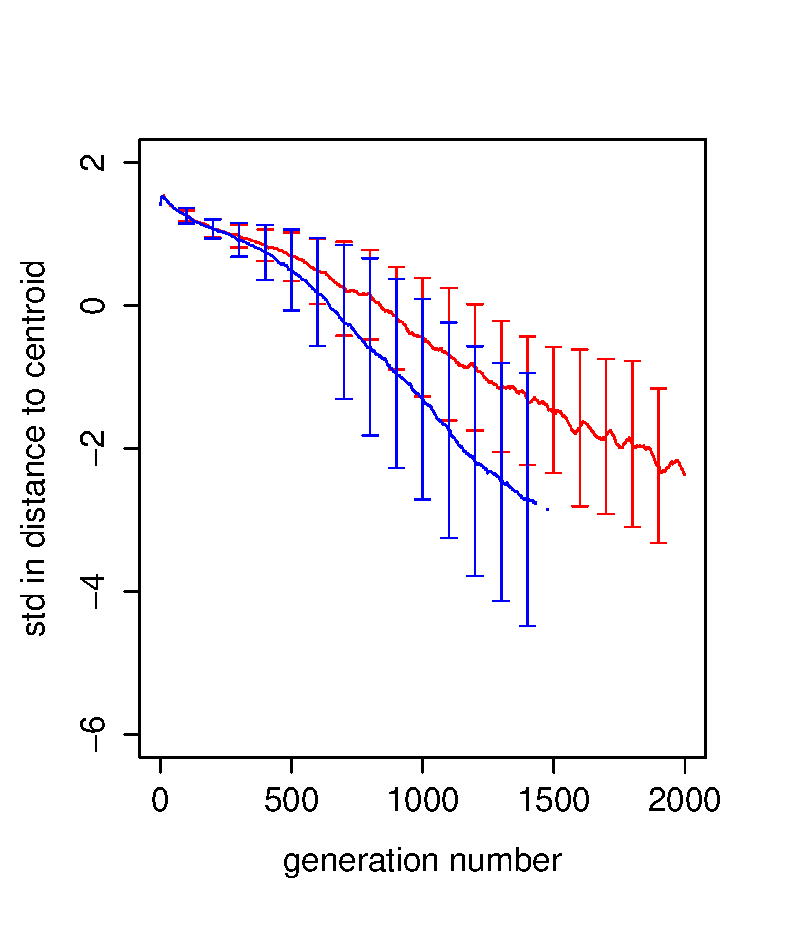
\includegraphics[clip, width=4.0cm]{P30D50.eps}
          \hspace{1.2cm} $P=30, D=50
$        \end{center}
      \end{minipage}

      % 3
      \begin{minipage}{0.33\hsize}
        \begin{center}
          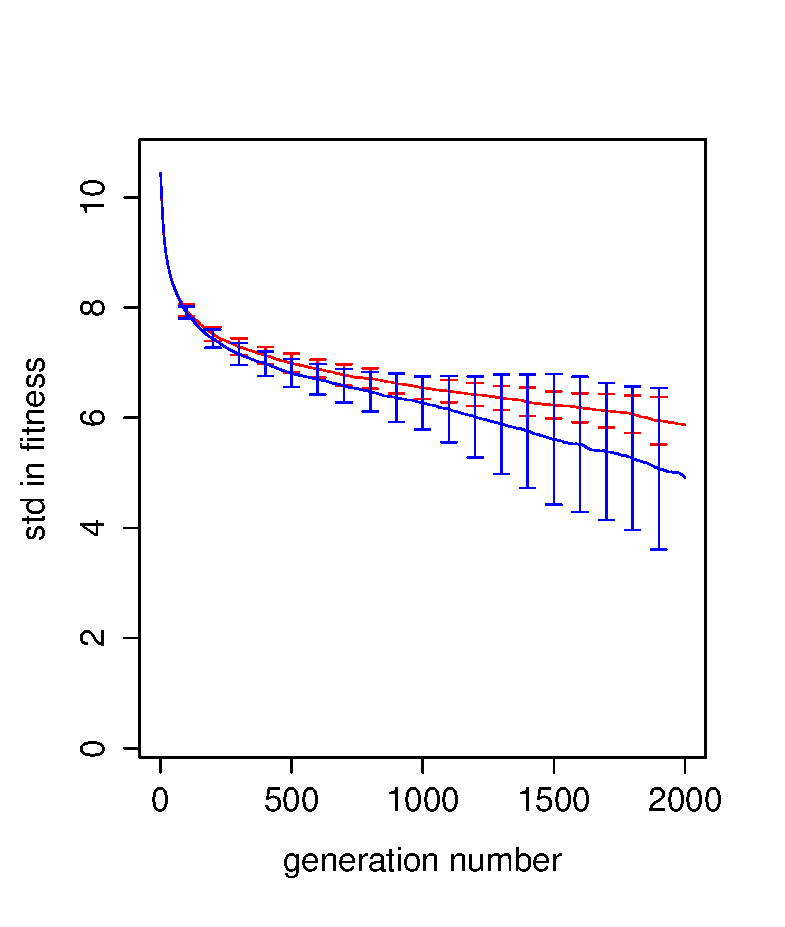
\includegraphics[clip, width=4.0cm]{P50D50.eps}
          \hspace{1.2cm} $P=50, D=50
$        \end{center}
      \end{minipage}
    \end{tabular}
  \end{center}
\end{figure}
\begin{figure}[htbp]
  \begin{center}
    \begin{tabular}{c}


      % 1
      \begin{minipage}{0.33\hsize}
        \begin{center}
          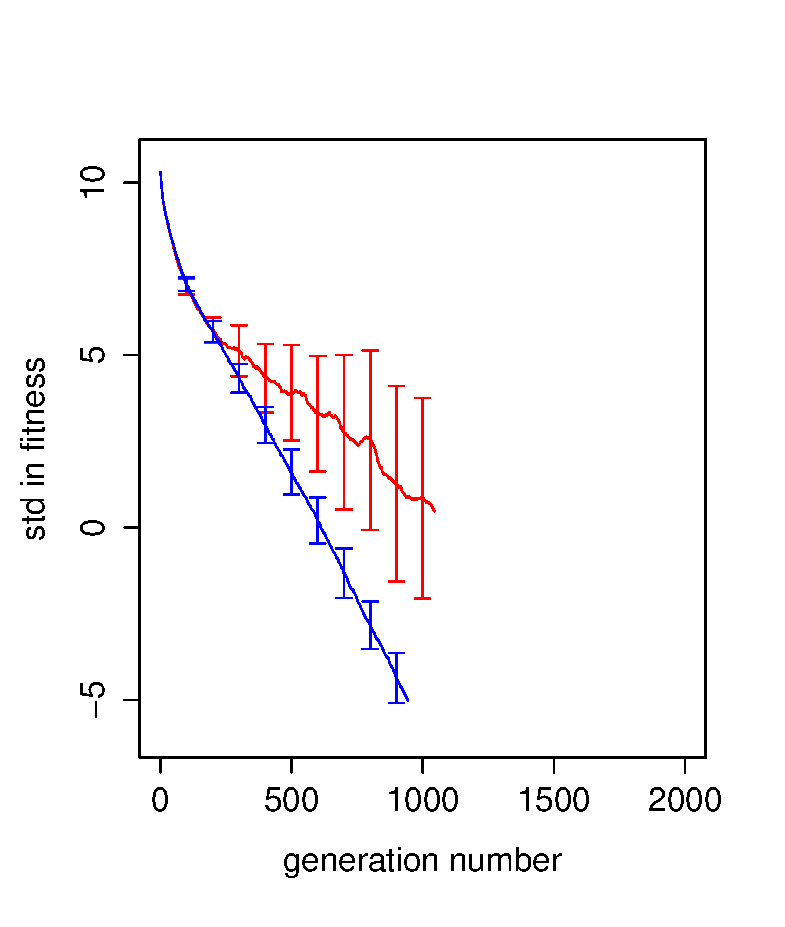
\includegraphics[clip, width=4.0cm]{P10D100.eps}
          \hspace{1.2cm} $P=10, D=100$
        \end{center}
      \end{minipage}

      % 2
      \begin{minipage}{0.33\hsize}
        \begin{center}
          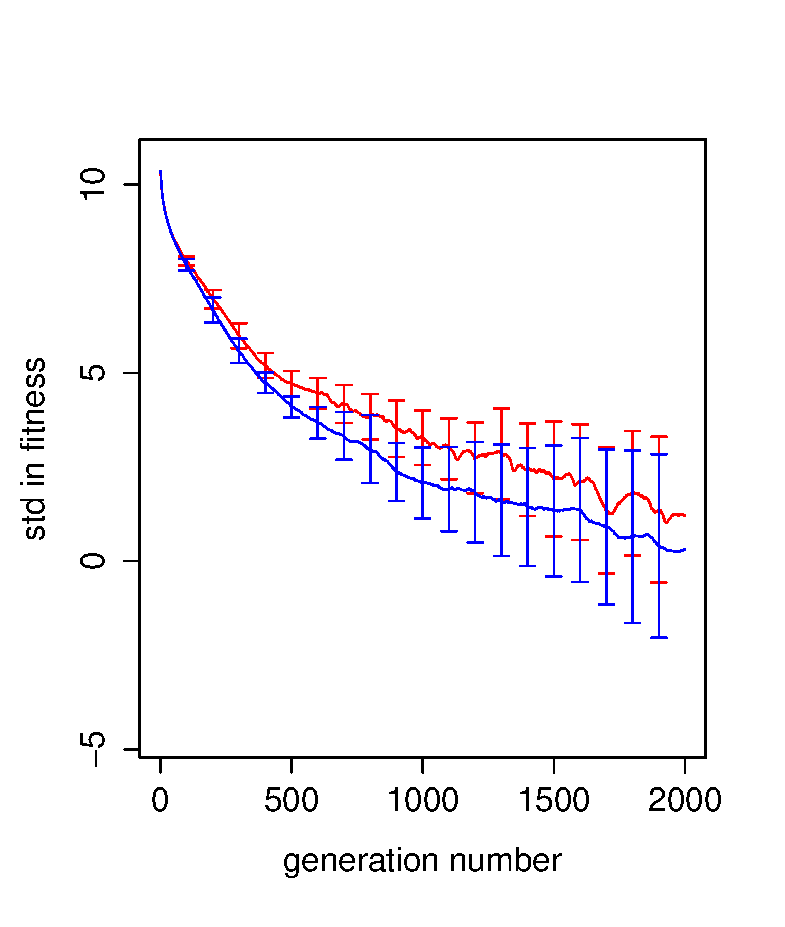
\includegraphics[clip, width=4.0cm]{P30D100.eps}
          \hspace{1.2cm} $P=30, D=100$
        \end{center}
      \end{minipage}

      % 3
      \begin{minipage}{0.33\hsize}
        \begin{center}
          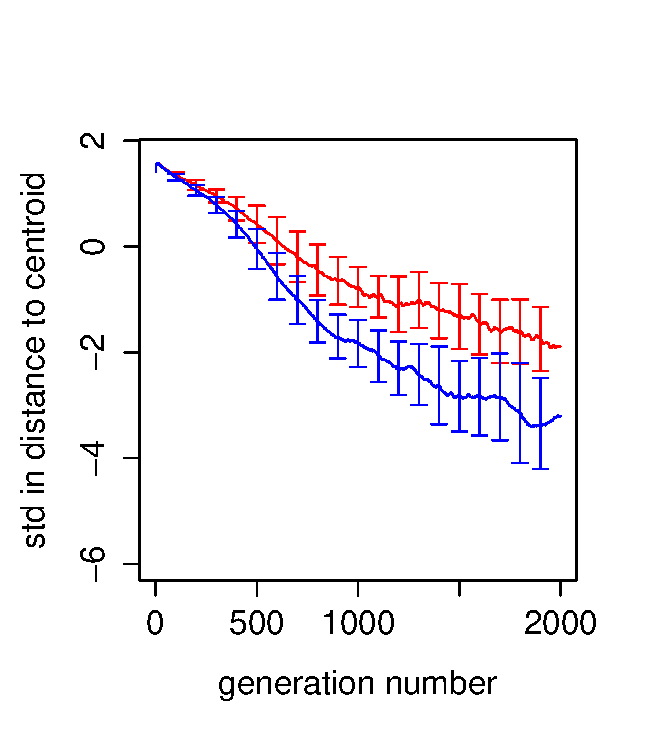
\includegraphics[clip, width=4.0cm]{P50D100.eps}
          \hspace{1.2cm} $P=50, D=100$
        \end{center}
      \end{minipage}
    \end{tabular}
    \label{fig:lena}
  \end{center}
\end{figure}

\newpage
% \caption{目的関数値による多様性維持の調査}
\begin{figure}[htbp]
  \caption{横軸は評価回数の経過を1から2000世代目まで表示している.縦軸は51回試行した多様性評価指標$r_f$について,平均値を求めそれに対し,常用対数をとったものである.DE/AとDE/NAの二つのアルゴリズムを用いて,それぞれ次元数$D$を$2,10,30,50,100$とし,集団数$P$を$10,30,50$とした時の多様性評価指標$r_f$が推移する様子を示している.}
  \begin{center}
    \begin{tabular}{c}


      % 1
      \begin{minipage}{0.33\hsize}
        \begin{center}
          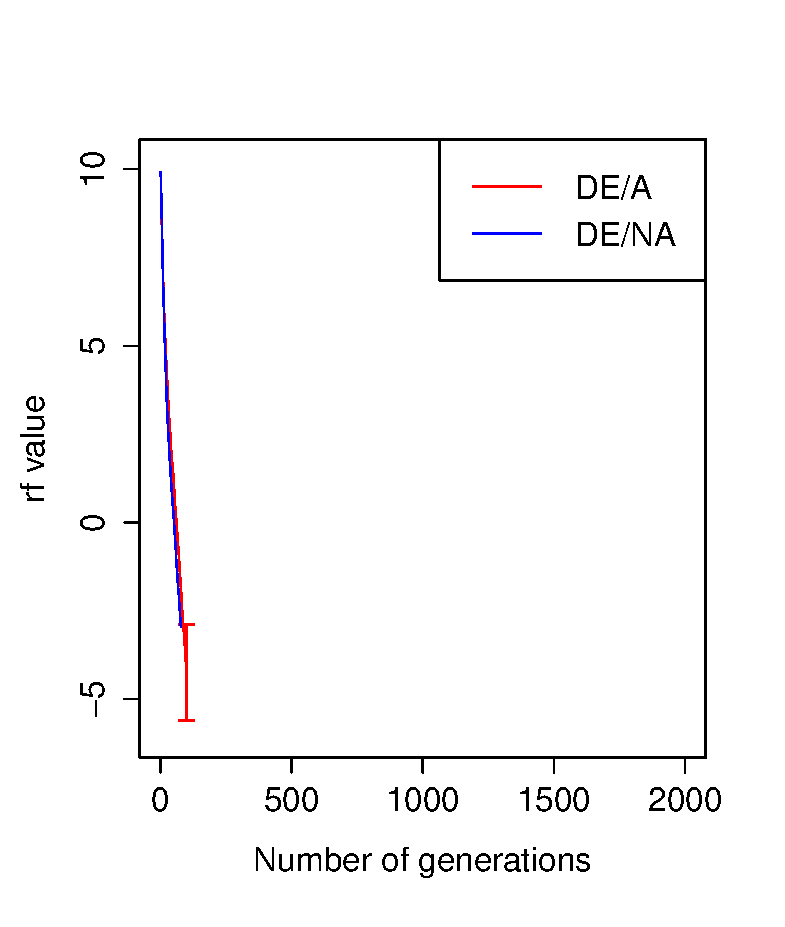
\includegraphics[clip, width=4.0cm]{P10fitD2.eps}
          \hspace{1.2cm}$P=10, D=2
 $       \end{center}
      \end{minipage}

      % 2
      \begin{minipage}{0.33\hsize}
        \begin{center}
          \includegraphics[clip, width=4.0cm]{P30fitD2.eps}
          \hspace{1.2cm}$P=30, D=2
 $       \end{center}
      \end{minipage}

      % 3
      \begin{minipage}{0.33\hsize}
        \begin{center}
          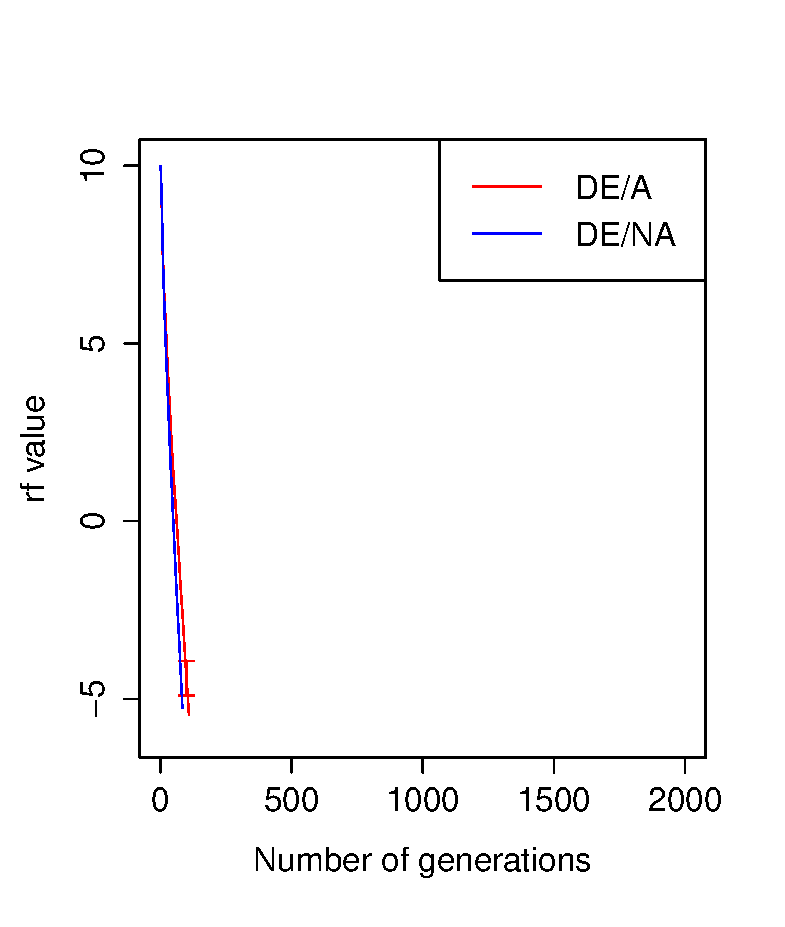
\includegraphics[clip, width=4.0cm]{P50fitD2.eps}
          \hspace{1.2cm}$P=50, D=2
 $       \end{center}
      \end{minipage}
    \end{tabular}
  \end{center}
\end{figure}
\begin{figure}[htbp]
  \begin{center}
    \begin{tabular}{c}


      % 1
      \begin{minipage}{0.33\hsize}
        \begin{center}
          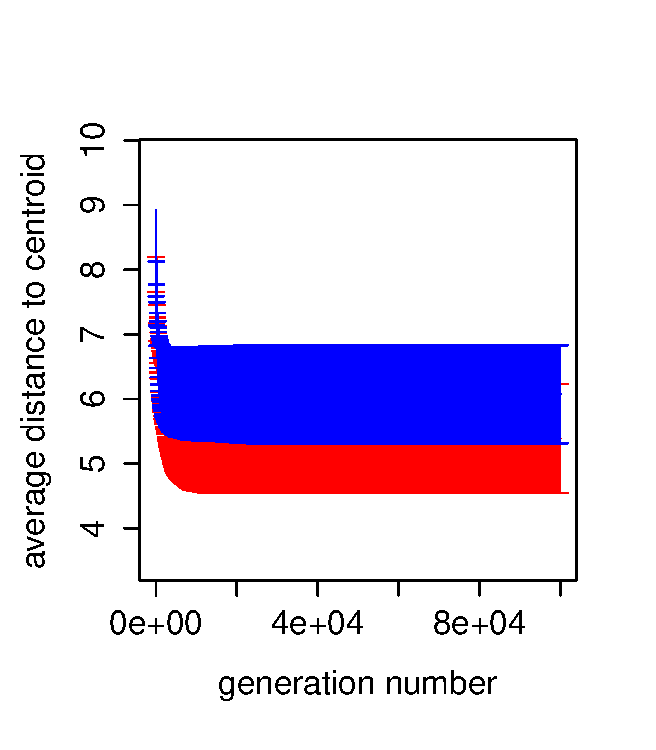
\includegraphics[clip, width=4.0cm]{P10fitD10.eps}
          \hspace{1.2cm}$P=10, D=10
$        \end{center}
      \end{minipage}

      % 2
      \begin{minipage}{0.33\hsize}
        \begin{center}
          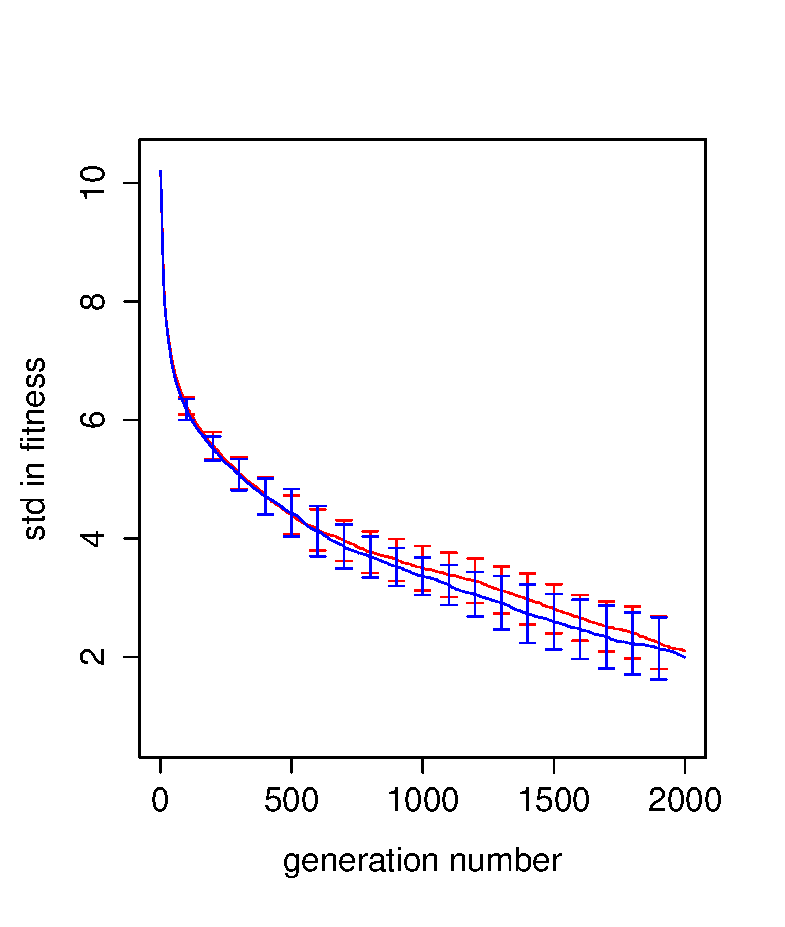
\includegraphics[clip, width=4.0cm]{P30fitD10.eps}
          \hspace{1.2cm}$P=30, D=10
$        \end{center}
      \end{minipage}

      % 3
      \begin{minipage}{0.33\hsize}
        \begin{center}
          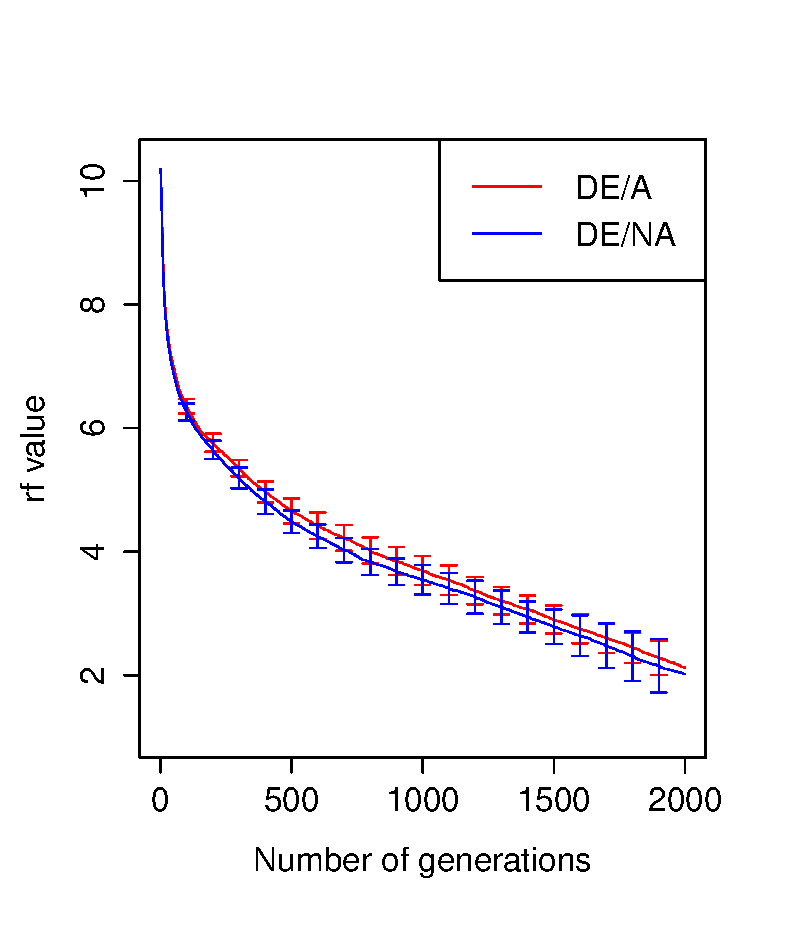
\includegraphics[clip, width=4.0cm]{P50fitD10.eps}
          \hspace{1.2cm}$P=50, D=10
$        \end{center}
      \end{minipage}
    \end{tabular}
  \end{center}
\end{figure}
\begin{figure}[htbp]
  \begin{center}
    \begin{tabular}{c}


      % 1
      \begin{minipage}{0.33\hsize}
        \begin{center}
          \includegraphics[clip, width=4.0cm]{P10fitD30.eps}
          \hspace{1.2cm}$P=10, D=30
$        \end{center}
      \end{minipage}

      % 2
      \begin{minipage}{0.33\hsize}
        \begin{center}
          \includegraphics[clip, width=4.0cm]{P30fitD30.eps}
          \hspace{1.2cm}$P=30, D=30
$        \end{center}
      \end{minipage}

      % 3
      \begin{minipage}{0.33\hsize}
        \begin{center}
          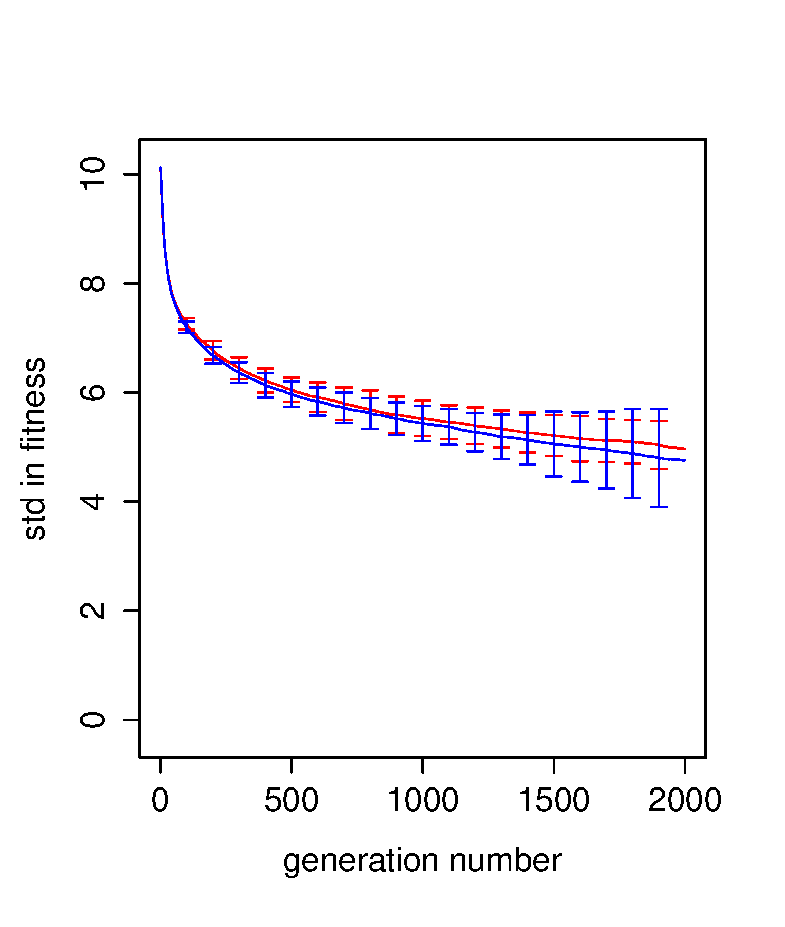
\includegraphics[clip, width=4.0cm]{P50fitD30.eps}
          \hspace{1.2cm}$P=50, D=30
$        \end{center}
      \end{minipage}
    \end{tabular}
  \end{center}
\end{figure}
\begin{figure}[htbp]
  \begin{center}
    \begin{tabular}{c}


      % 1
      \begin{minipage}{0.33\hsize}
        \begin{center}
          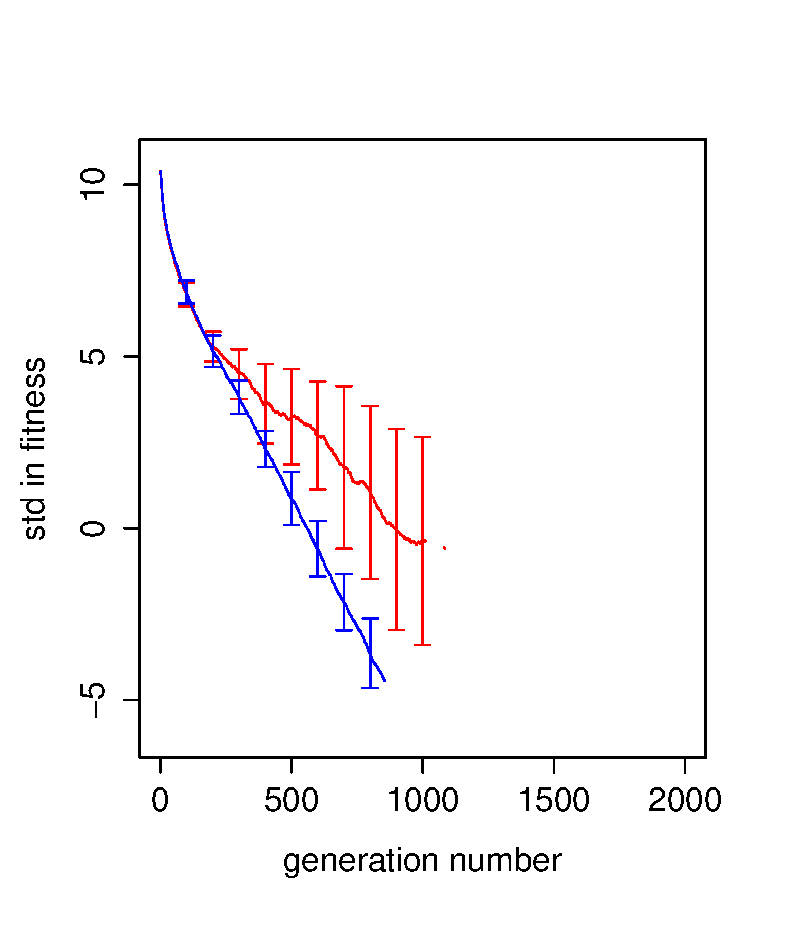
\includegraphics[clip, width=4.0cm]{P10fitD50.eps}
          \hspace{1.2cm} $P=10, D=50
$        \end{center}
      \end{minipage}

      % 2
      \begin{minipage}{0.33\hsize}
        \begin{center}
          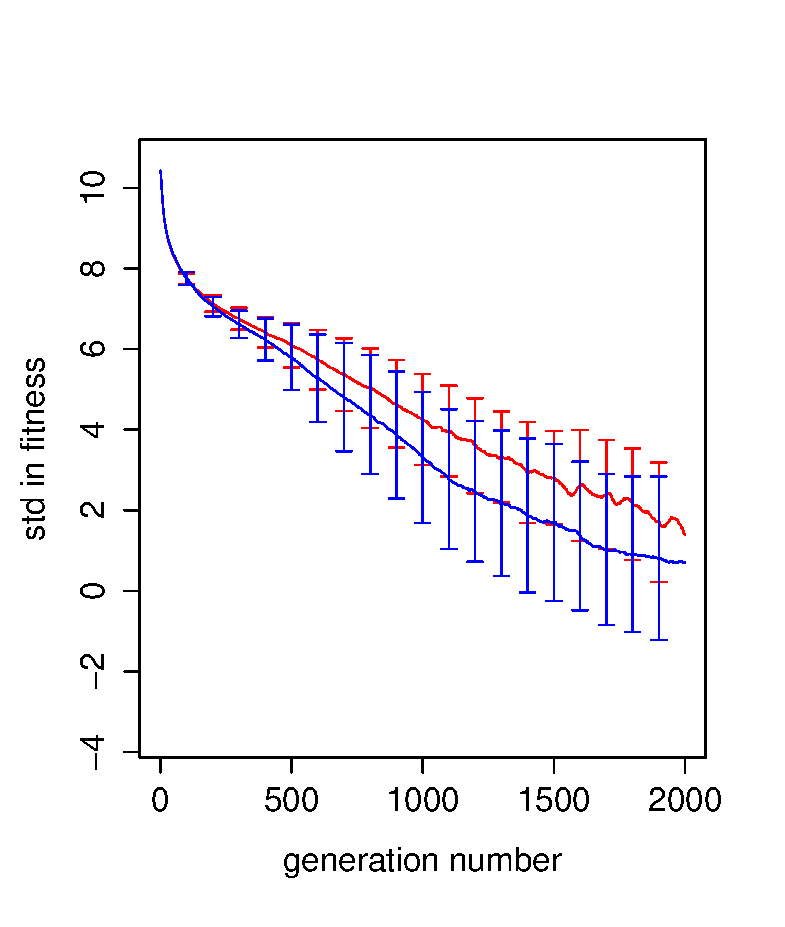
\includegraphics[clip, width=4.0cm]{P30fitD50.eps}
          \hspace{1.2cm} $P=30, D=50
$        \end{center}
      \end{minipage}

      % 3
      \begin{minipage}{0.33\hsize}
        \begin{center}
          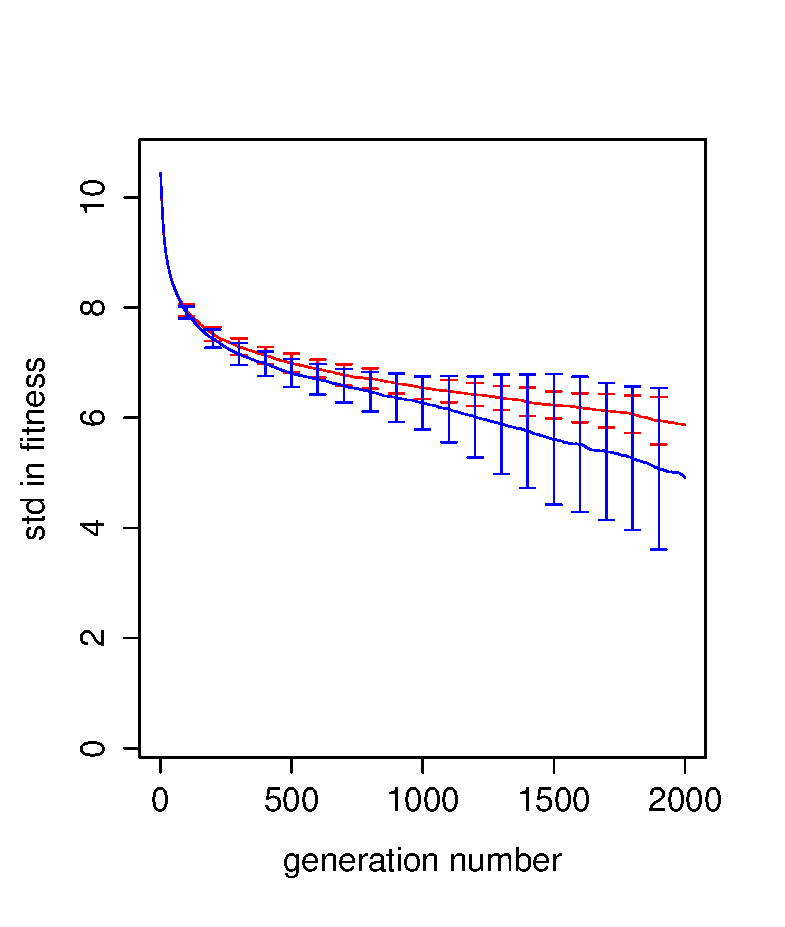
\includegraphics[clip, width=4.0cm]{P50fitD50.eps}
          \hspace{1.2cm} $P=50, D=50
$        \end{center}
      \end{minipage}
    \end{tabular}
  \end{center}
\end{figure}
\begin{figure}[htbp]
  \begin{center}
    \begin{tabular}{c}

      % 1
      \begin{minipage}{0.33\hsize}
        \begin{center}
          \includegraphics[clip, width=4.0cm]{P10fitD100.eps}
          \hspace{1.2cm} $P=10, D=100$
        \end{center}
      \end{minipage}

      % 2
      \begin{minipage}{0.33\hsize}
        \begin{center}
          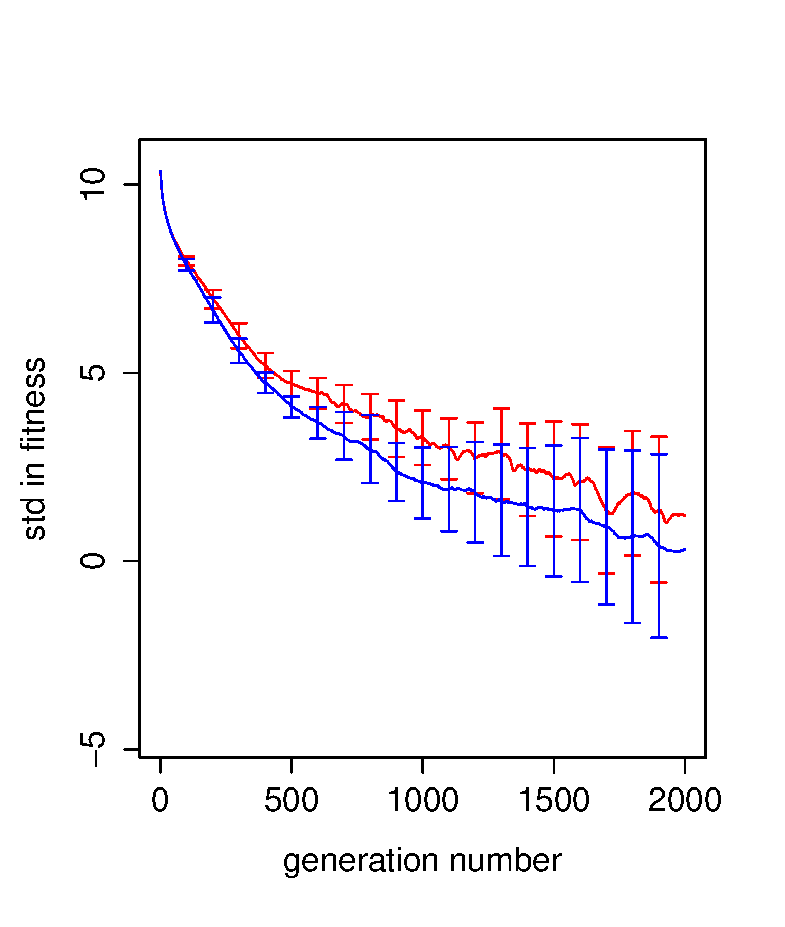
\includegraphics[clip, width=4.0cm]{P30fitD100.eps}
          \hspace{1.2cm} $P=30, D=100$
        \end{center}
      \end{minipage}

      % 3
      \begin{minipage}{0.33\hsize}
        \begin{center}
          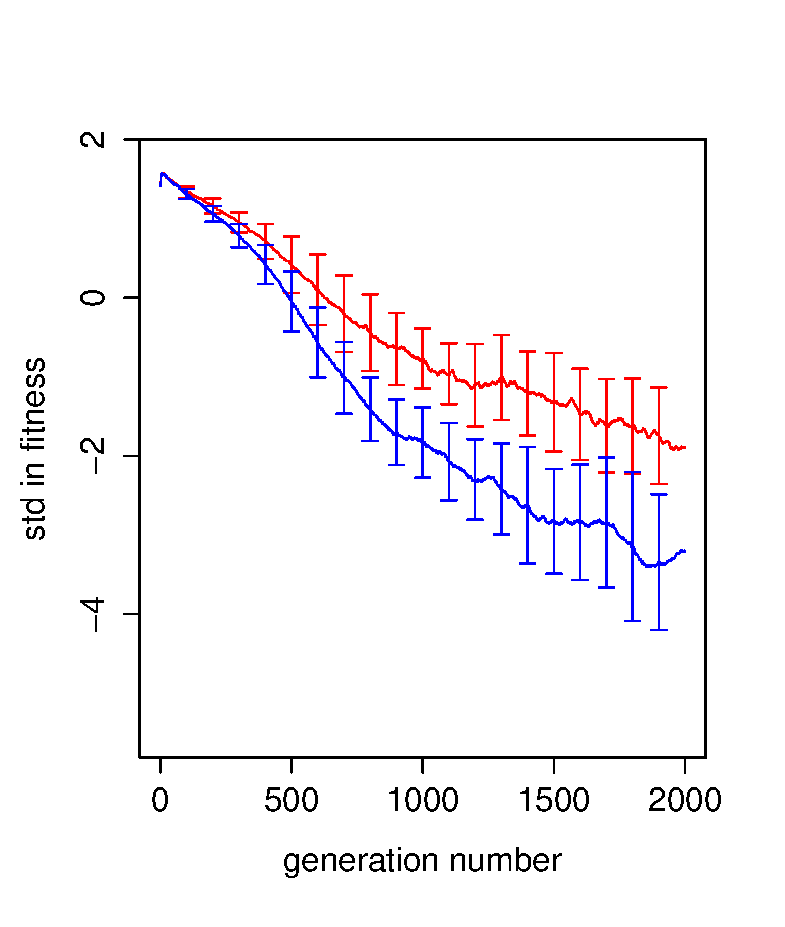
\includegraphics[clip, width=4.0cm]{P50fitD100.eps}
          \hspace{1.2cm} $P=50, D=100$
        \end{center}
      \end{minipage}
    \end{tabular}
    \label{fig:lena}
  \end{center}
\end{figure}

\newpage
\begin{figure}[htbp]
  \caption{横軸は評価回数の経過を1から2000世代目まで表示している.縦軸は51回試行した多様性評価指標$r_s$について,平均値を求めそれに対し,常用対数をとったものである.DE/AとDE/NAの二つのアルゴリズムを用いて,それぞれ次元数$D$を$2,10,30,50,100$とし,集団数$P$を$10,30,50$とした時の多様性評価指標$r_s$が推移する様子を示している.}
  \begin{center}
    \begin{tabular}{c}
      % 1
      \begin{minipage}{0.33\hsize}
        \begin{center}
          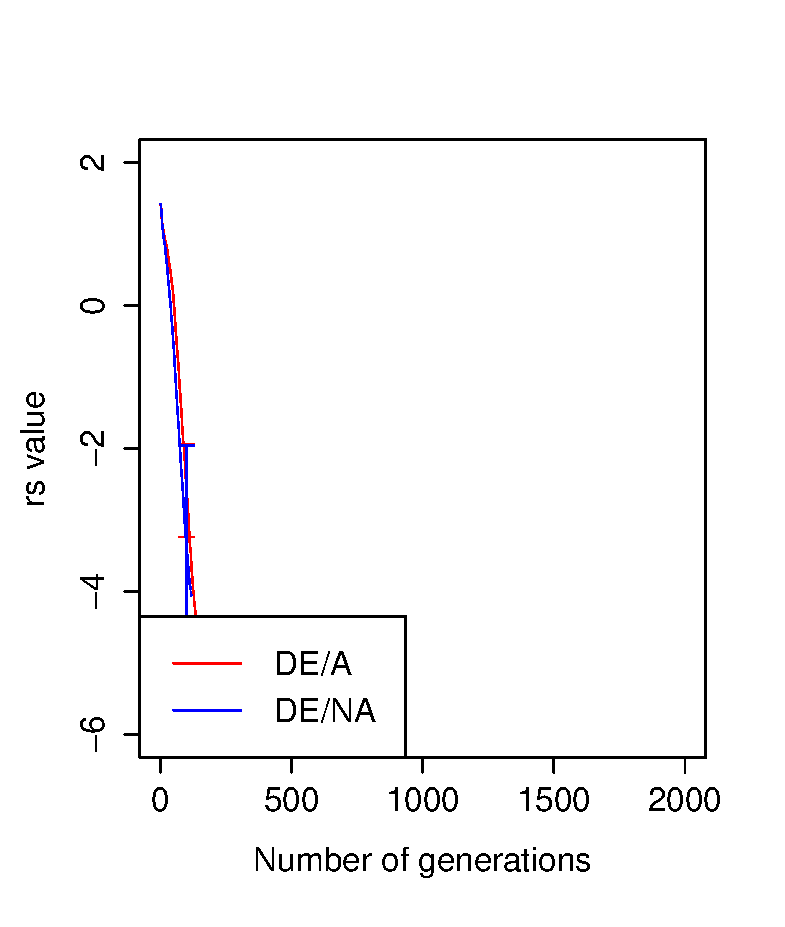
\includegraphics[clip, width=4.0cm]{P10D2.eps}
          \hspace{1.2cm}$P=10, D=2
 $       \end{center}
      \end{minipage}

      % 2
      \begin{minipage}{0.33\hsize}
        \begin{center}
          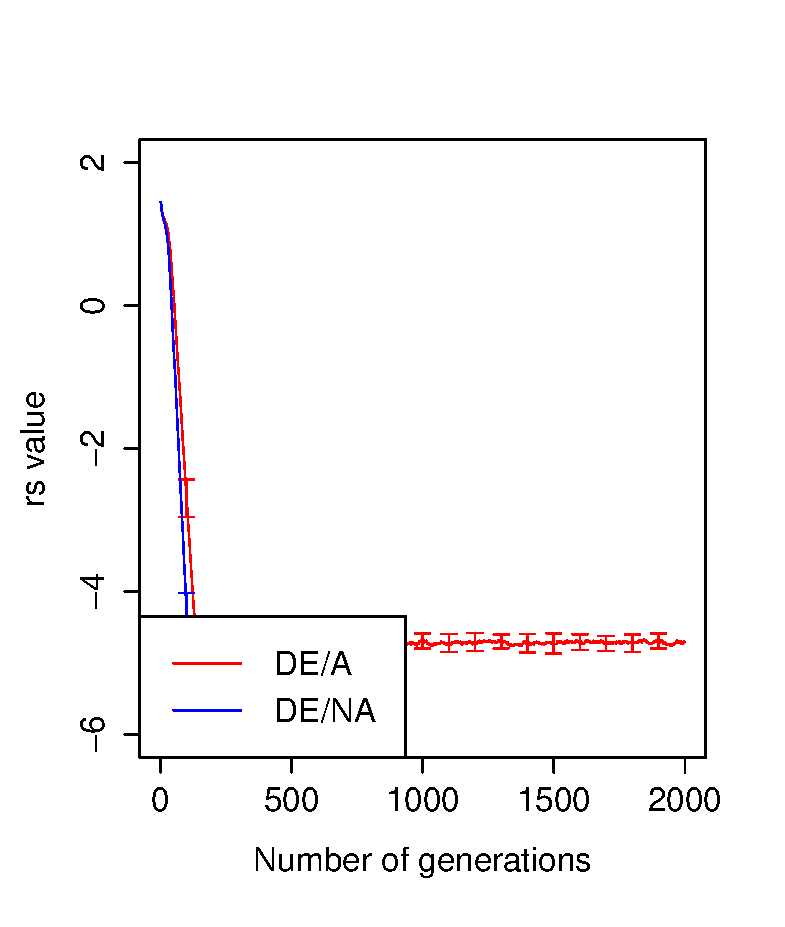
\includegraphics[clip, width=4.0cm]{P30D2.eps}
          \hspace{1.2cm}$P=30, D=2
 $       \end{center}
      \end{minipage}

      % 3
      \begin{minipage}{0.33\hsize}
        \begin{center}
          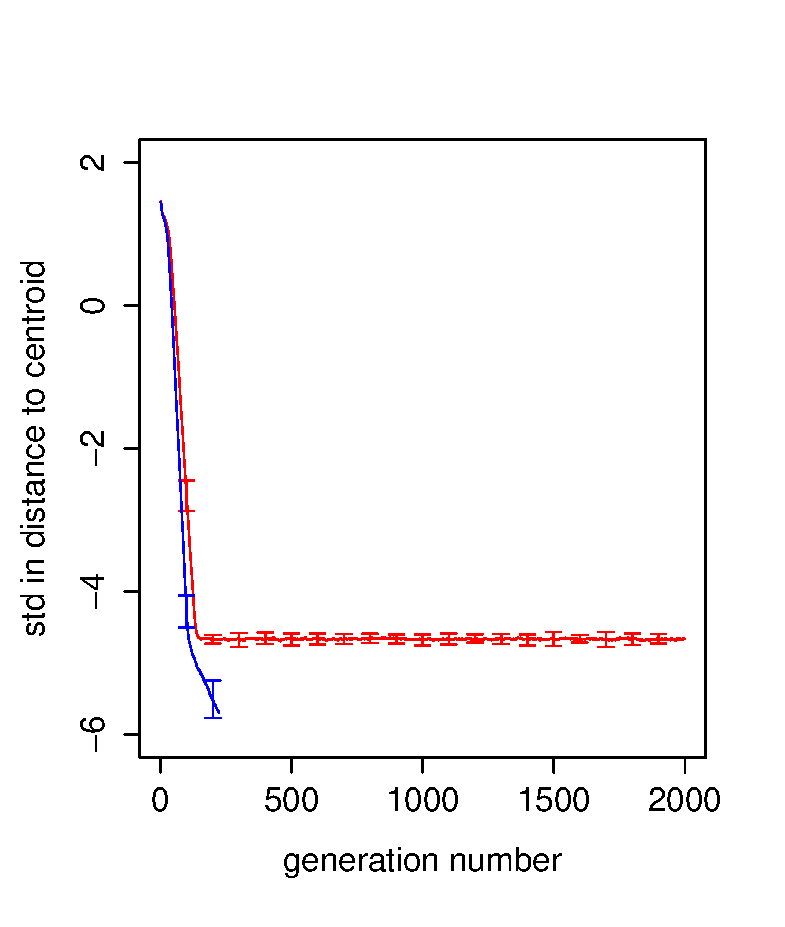
\includegraphics[clip, width=4.0cm]{P50D2.eps}
          \hspace{1.2cm}$P=50, D=2
 $       \end{center}
      \end{minipage}
    \end{tabular}
  \end{center}
\end{figure}
\begin{figure}[htbp]
  \begin{center}
    \begin{tabular}{c}


      % 1
      \begin{minipage}{0.33\hsize}
        \begin{center}
          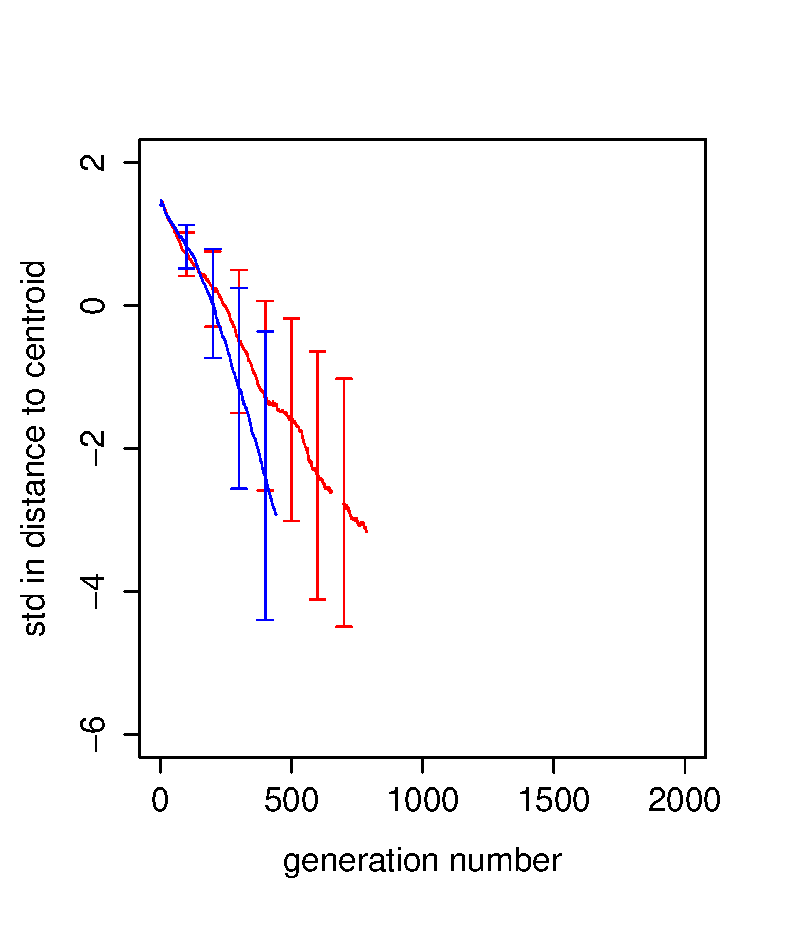
\includegraphics[clip, width=4.0cm]{P10D10.eps}
          \hspace{1.2cm}$P=10, D=10
$        \end{center}
      \end{minipage}

      % 2
      \begin{minipage}{0.33\hsize}
        \begin{center}
          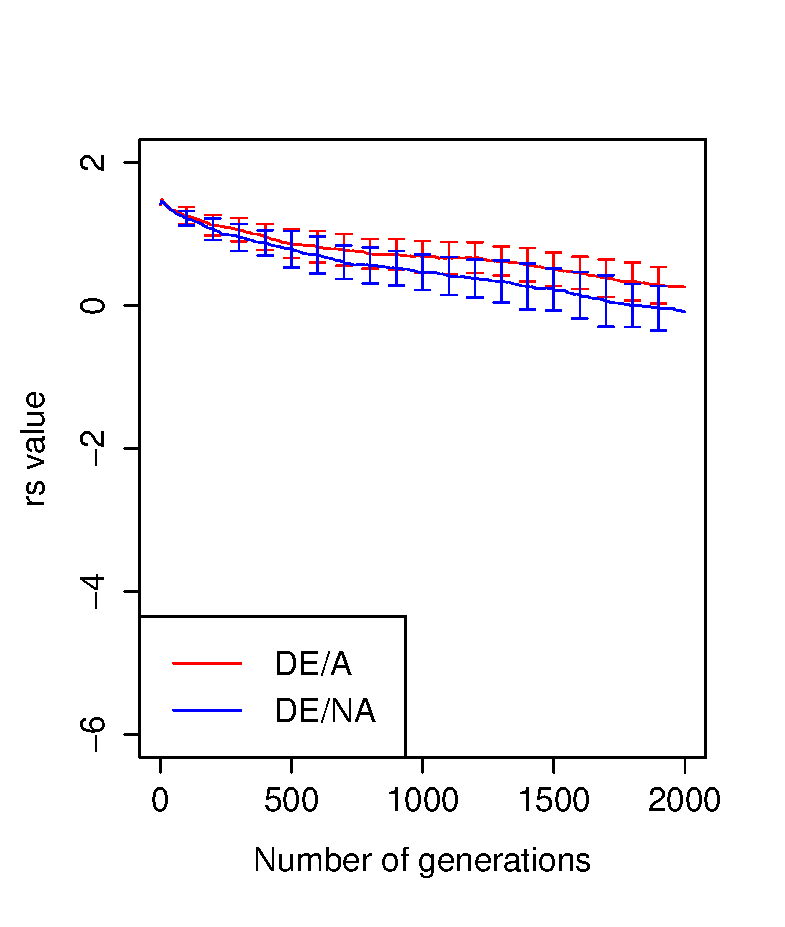
\includegraphics[clip, width=4.0cm]{P30D10.eps}
          \hspace{1.2cm}$P=30, D=10
$        \end{center}
      \end{minipage}

      % 3
      \begin{minipage}{0.33\hsize}
        \begin{center}
          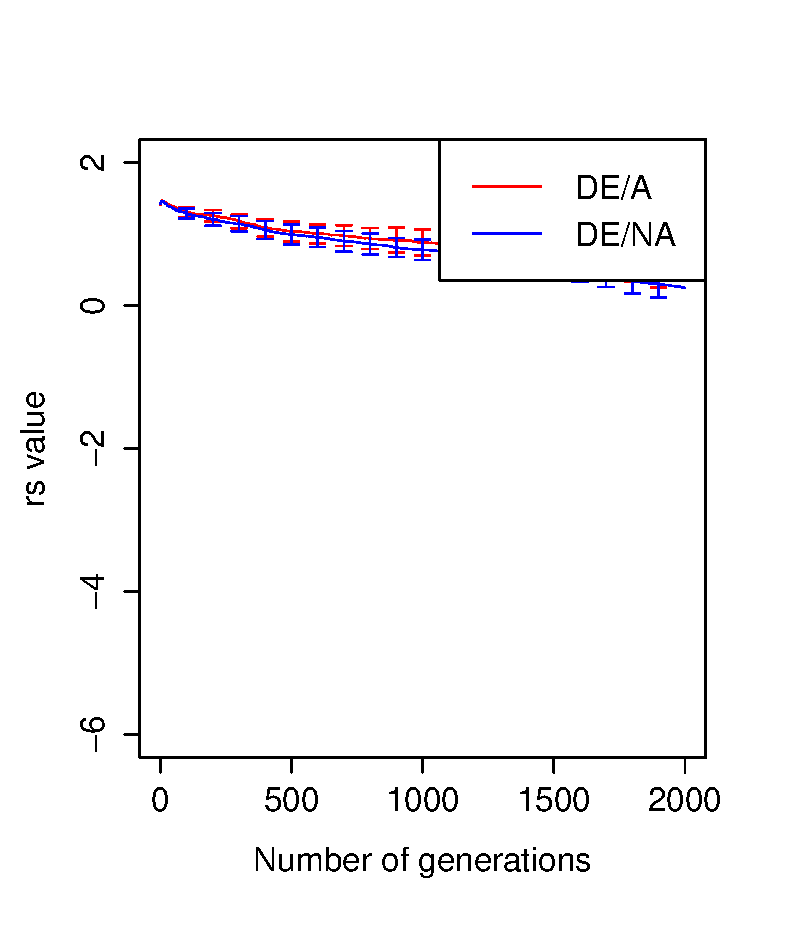
\includegraphics[clip, width=4.0cm]{P50D10.eps}
          \hspace{1.2cm}$P=50, D=10
$        \end{center}
      \end{minipage}
    \end{tabular}
  \end{center}
\end{figure}
\begin{figure}[htbp]
  \begin{center}
    \begin{tabular}{c}


      % 1
      \begin{minipage}{0.33\hsize}
        \begin{center}
          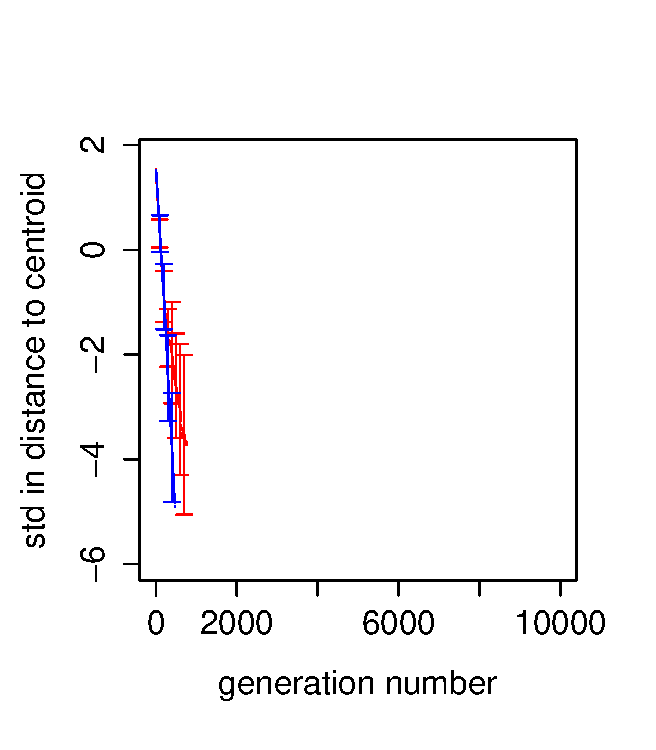
\includegraphics[clip, width=4.0cm]{P10D30.eps}
          \hspace{1.2cm}$P=10, D=30
$        \end{center}
      \end{minipage}

      % 2
      \begin{minipage}{0.33\hsize}
        \begin{center}
          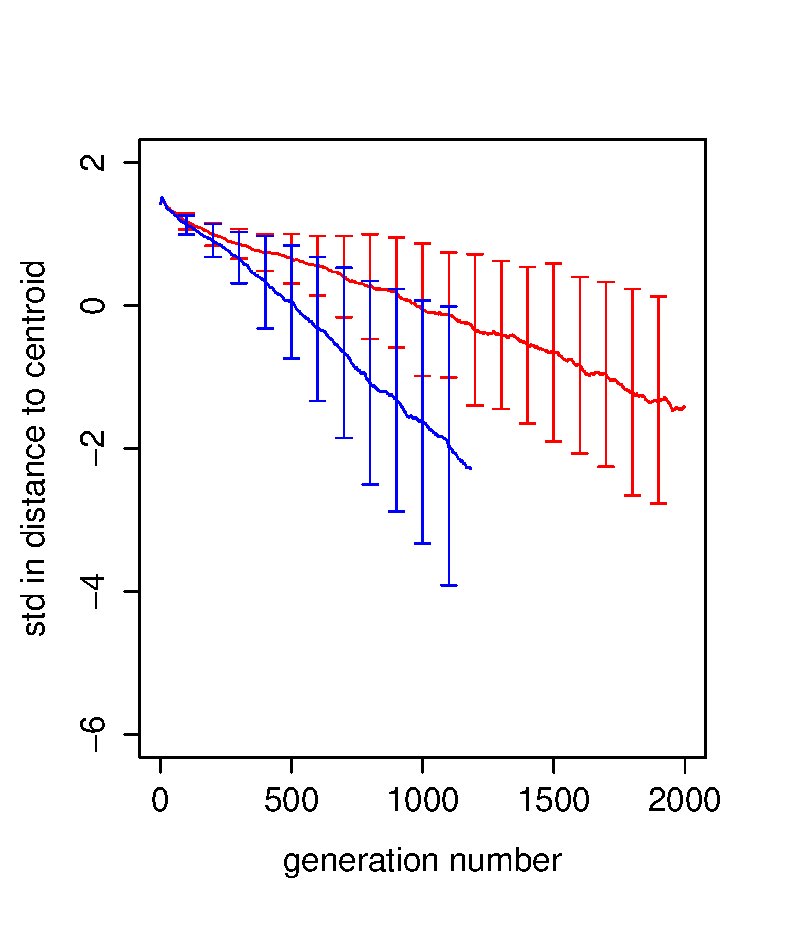
\includegraphics[clip, width=4.0cm]{P30D30.eps}
          \hspace{1.2cm}$P=30, D=30
$        \end{center}
      \end{minipage}

      % 3
      \begin{minipage}{0.33\hsize}
        \begin{center}
          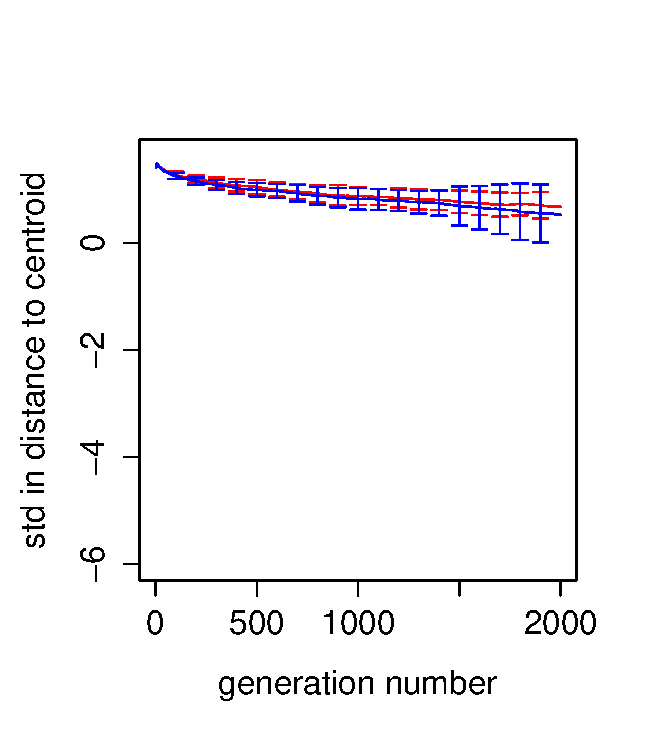
\includegraphics[clip, width=4.0cm]{P50D30.eps}
          \hspace{1.2cm}$P=50, D=30
$        \end{center}
      \end{minipage}
    \end{tabular}
  \end{center}
\end{figure}
\begin{figure}[htbp]
  \begin{center}
    \begin{tabular}{c}


      % 1
      \begin{minipage}{0.33\hsize}
        \begin{center}
          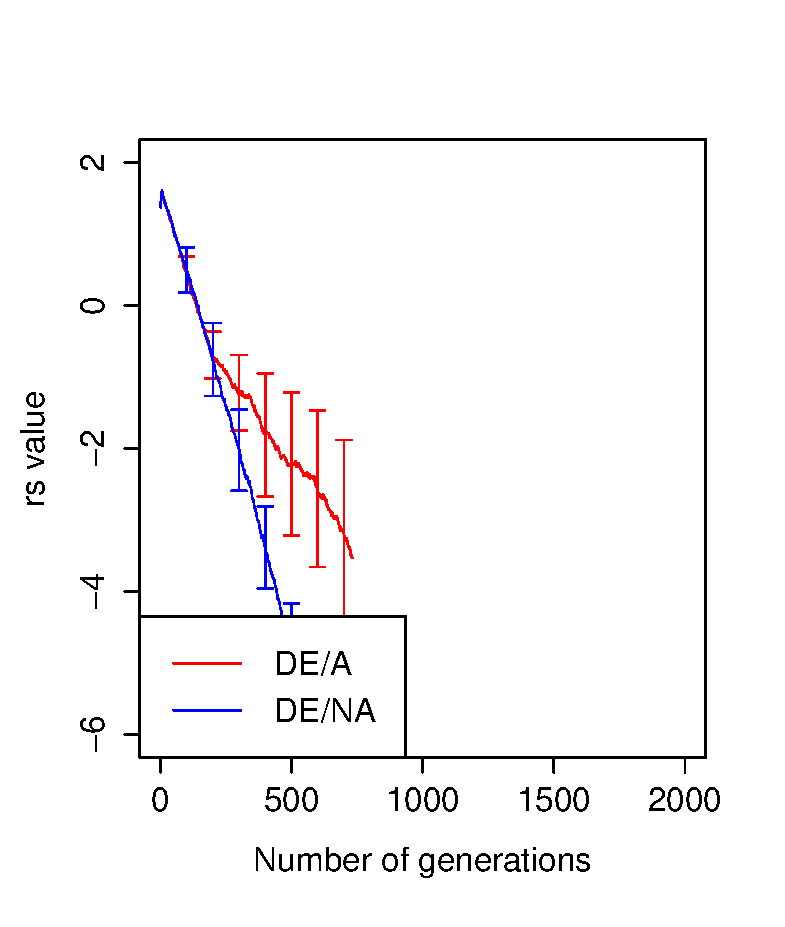
\includegraphics[clip, width=4.0cm]{P10D50.eps}
          \hspace{1.2cm} $P=10, D=50
$        \end{center}
      \end{minipage}

      % 2
      \begin{minipage}{0.33\hsize}
        \begin{center}
          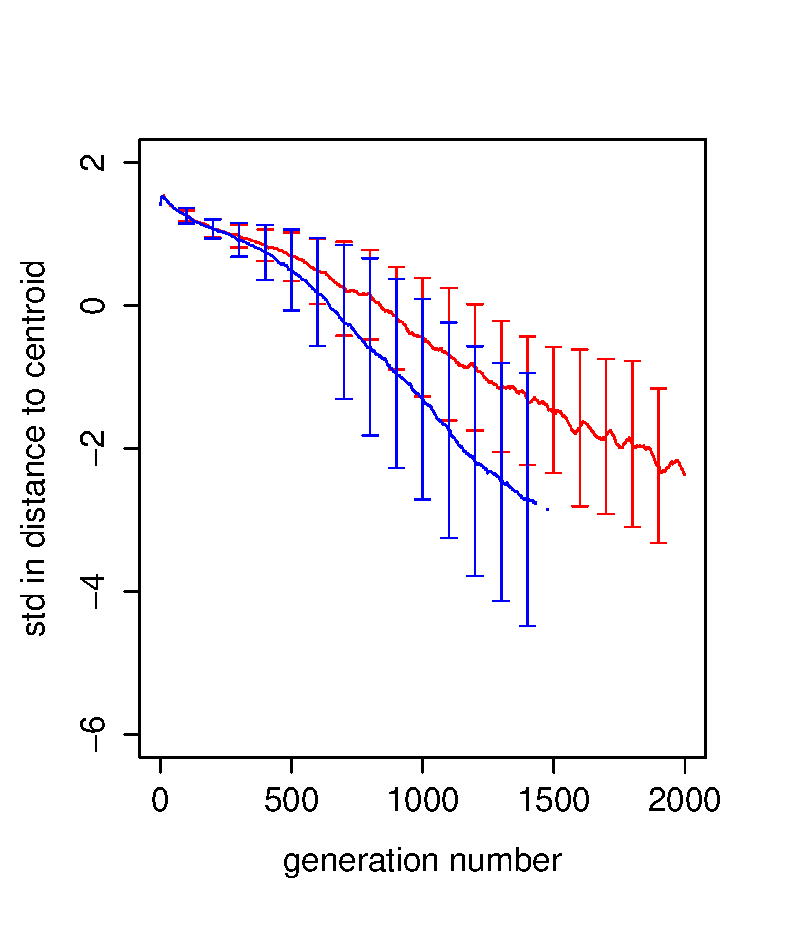
\includegraphics[clip, width=4.0cm]{P30D50.eps}
          \hspace{1.2cm} $P=30, D=50
$        \end{center}
      \end{minipage}

      % 3
      \begin{minipage}{0.33\hsize}
        \begin{center}
          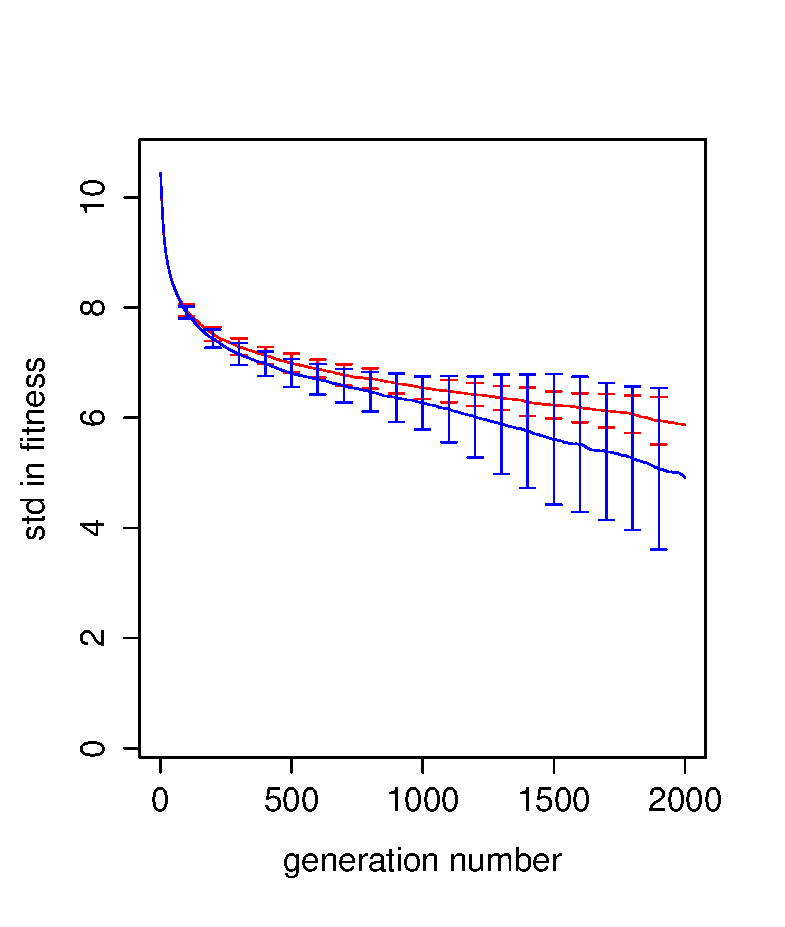
\includegraphics[clip, width=4.0cm]{P50D50.eps}
          \hspace{1.2cm} $P=50, D=50
$        \end{center}
      \end{minipage}
    \end{tabular}
  \end{center}
\end{figure}
\begin{figure}[htbp]
  \begin{center}
    \begin{tabular}{c}


      % 1
      \begin{minipage}{0.33\hsize}
        \begin{center}
          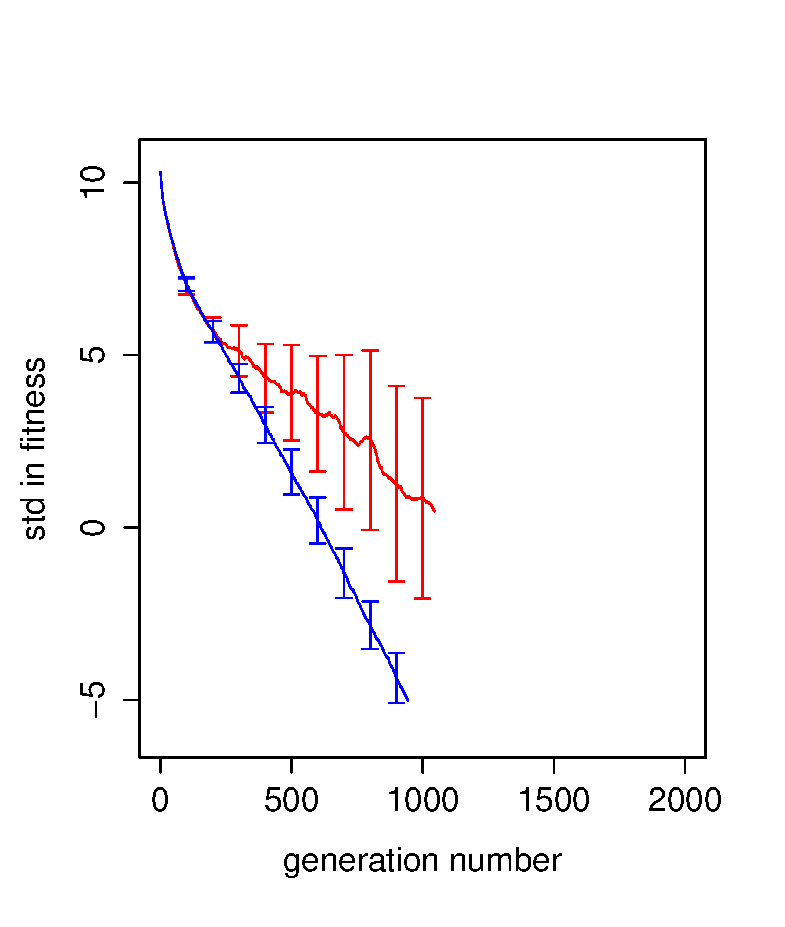
\includegraphics[clip, width=4.0cm]{P10D100.eps}
          \hspace{1.2cm} $P=10, D=100$
        \end{center}
      \end{minipage}

      % 2
      \begin{minipage}{0.33\hsize}
        \begin{center}
          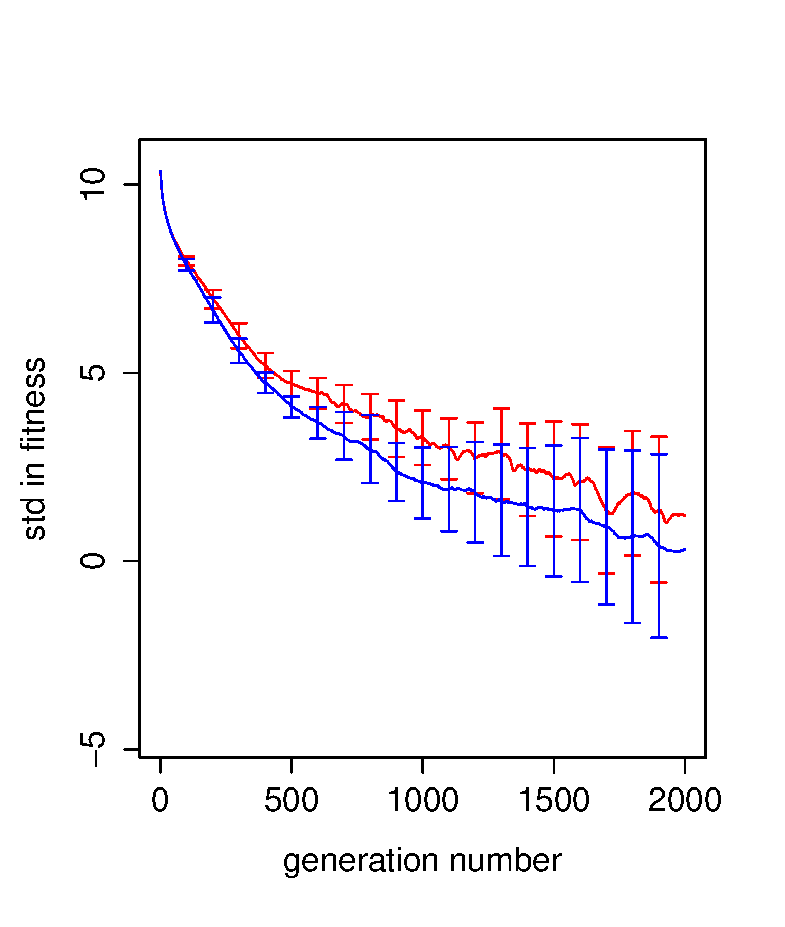
\includegraphics[clip, width=4.0cm]{P30D100.eps}
          \hspace{1.2cm} $P=30, D=100$
        \end{center}
      \end{minipage}

      % 3
      \begin{minipage}{0.33\hsize}
        \begin{center}
          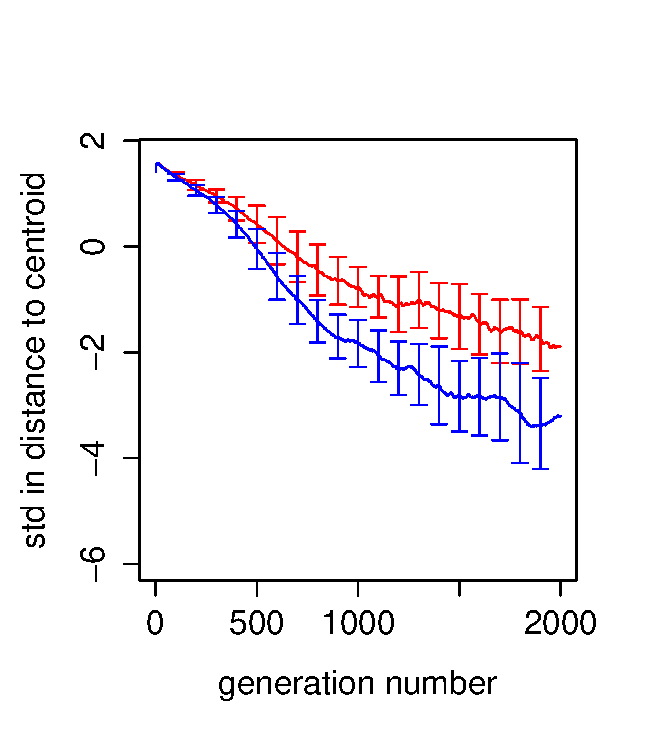
\includegraphics[clip, width=4.0cm]{P50D100.eps}
          \hspace{1.2cm} $P=50, D=100$
        \end{center}
      \end{minipage}
    \end{tabular}
    \label{fig:lena}
  \end{center}
\end{figure}

\newpage
% \caption{目的関数値による多様性維持の調査}
\begin{figure}[htbp]
  \caption{横軸は評価回数の経過を1から2000世代目まで表示している.縦軸は51回試行した多様性評価指標$r_f$について,平均値を求めそれに対し,常用対数をとったものである.DE/AとDE/NAの二つのアルゴリズムを用いて,それぞれ次元数$D$を$2,10,30,50,100$とし,集団数$P$を$10,30,50$とした時の多様性評価指標$r_f$が推移する様子を示している.}
  \begin{center}
    \begin{tabular}{c}


      % 1
      \begin{minipage}{0.33\hsize}
        \begin{center}
          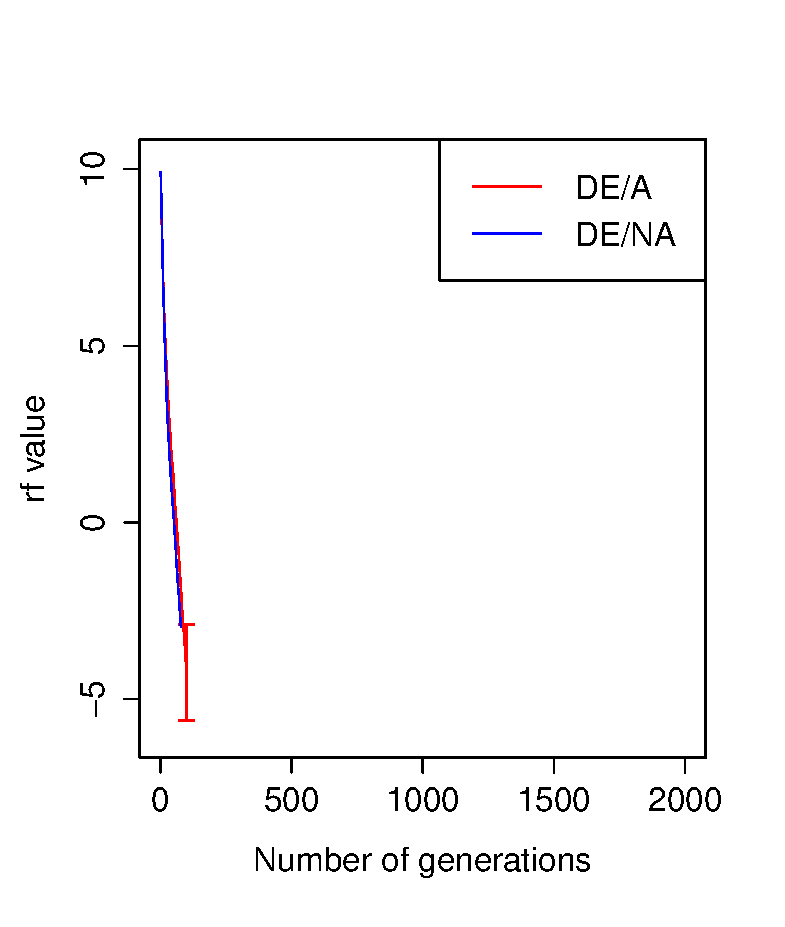
\includegraphics[clip, width=4.0cm]{P10fitD2.eps}
          \hspace{1.2cm}$P=10, D=2
 $       \end{center}
      \end{minipage}

      % 2
      \begin{minipage}{0.33\hsize}
        \begin{center}
          \includegraphics[clip, width=4.0cm]{P30fitD2.eps}
          \hspace{1.2cm}$P=30, D=2
 $       \end{center}
      \end{minipage}

      % 3
      \begin{minipage}{0.33\hsize}
        \begin{center}
          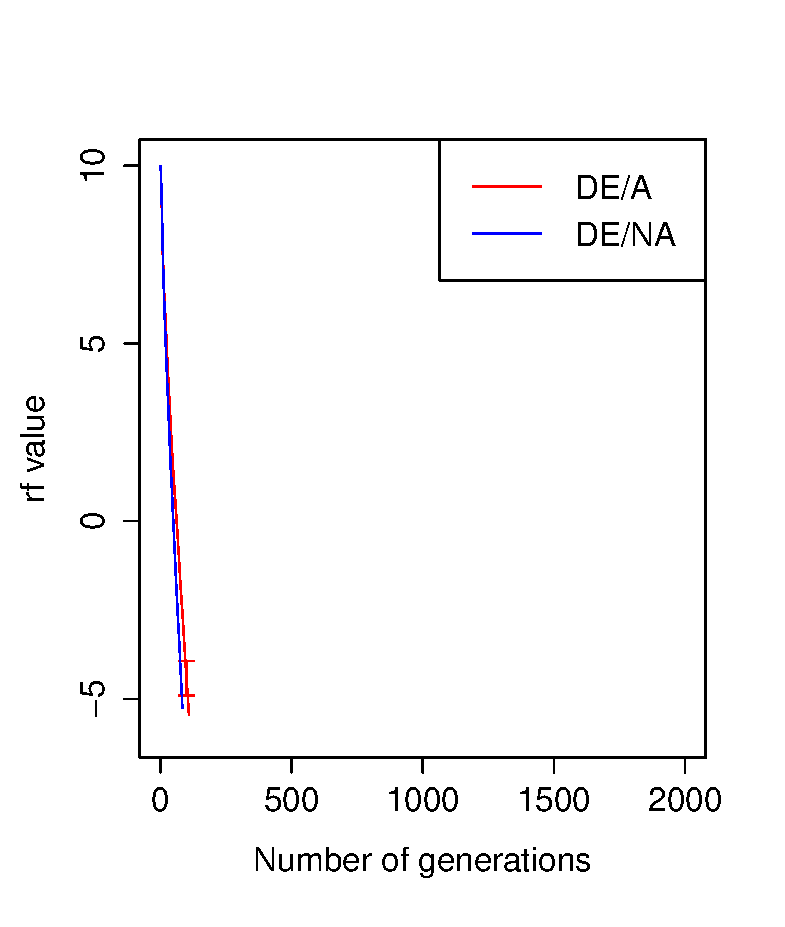
\includegraphics[clip, width=4.0cm]{P50fitD2.eps}
          \hspace{1.2cm}$P=50, D=2
 $       \end{center}
      \end{minipage}
    \end{tabular}
  \end{center}
\end{figure}
\begin{figure}[htbp]
  \begin{center}
    \begin{tabular}{c}


      % 1
      \begin{minipage}{0.33\hsize}
        \begin{center}
          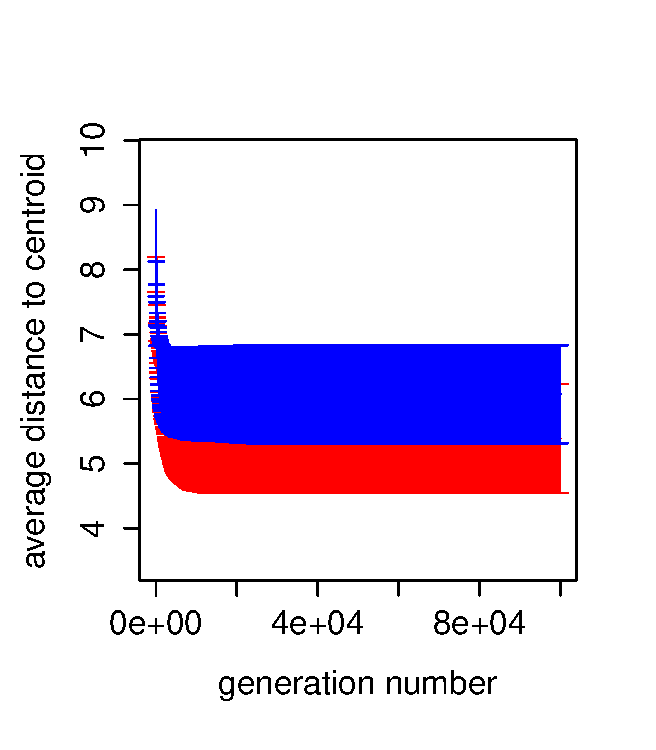
\includegraphics[clip, width=4.0cm]{P10fitD10.eps}
          \hspace{1.2cm}$P=10, D=10
$        \end{center}
      \end{minipage}

      % 2
      \begin{minipage}{0.33\hsize}
        \begin{center}
          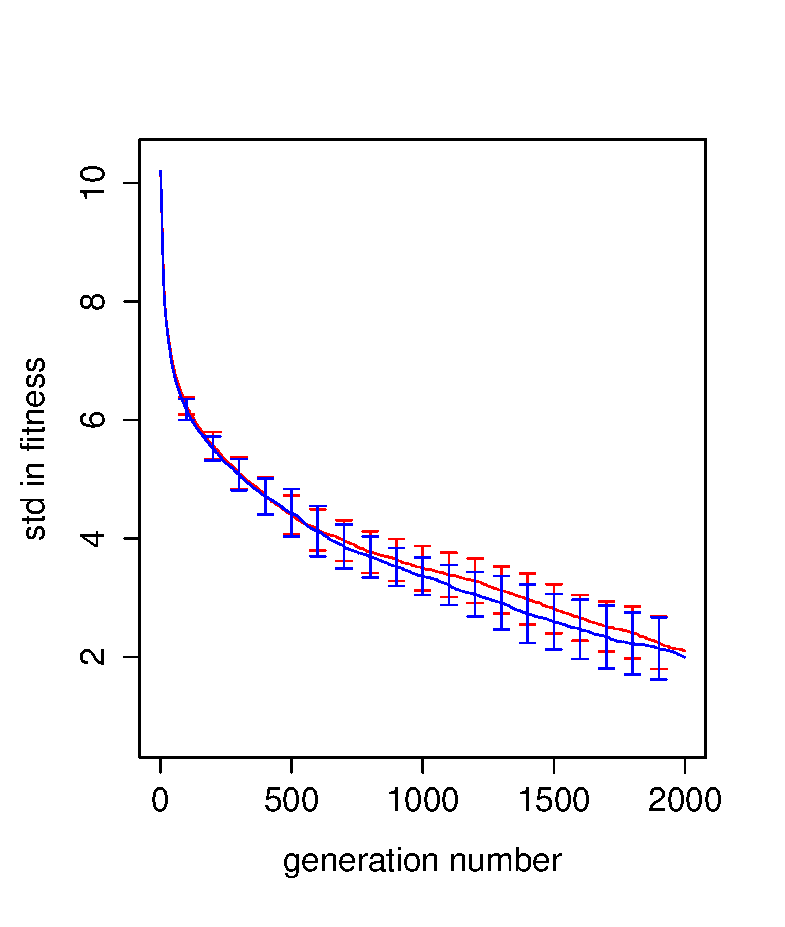
\includegraphics[clip, width=4.0cm]{P30fitD10.eps}
          \hspace{1.2cm}$P=30, D=10
$        \end{center}
      \end{minipage}

      % 3
      \begin{minipage}{0.33\hsize}
        \begin{center}
          \includegraphics[clip, width=4.0cm]{P50fitD10.eps}
          \hspace{1.2cm}$P=50, D=10
$        \end{center}
      \end{minipage}
    \end{tabular}
  \end{center}
\end{figure}
\begin{figure}[htbp]
  \begin{center}
    \begin{tabular}{c}


      % 1
      \begin{minipage}{0.33\hsize}
        \begin{center}
          \includegraphics[clip, width=4.0cm]{P10fitD30.eps}
          \hspace{1.2cm}$P=10, D=30
$        \end{center}
      \end{minipage}

      % 2
      \begin{minipage}{0.33\hsize}
        \begin{center}
          \includegraphics[clip, width=4.0cm]{P30fitD30.eps}
          \hspace{1.2cm}$P=30, D=30
$        \end{center}
      \end{minipage}

      % 3
      \begin{minipage}{0.33\hsize}
        \begin{center}
          \includegraphics[clip, width=4.0cm]{P50fitD30.eps}
          \hspace{1.2cm}$P=50, D=30
$        \end{center}
      \end{minipage}
    \end{tabular}
  \end{center}
\end{figure}
\begin{figure}[htbp]
  \begin{center}
    \begin{tabular}{c}


      % 1
      \begin{minipage}{0.33\hsize}
        \begin{center}
          \includegraphics[clip, width=4.0cm]{P10fitD50.eps}
          \hspace{1.2cm} $P=10, D=50
$        \end{center}
      \end{minipage}

      % 2
      \begin{minipage}{0.33\hsize}
        \begin{center}
          \includegraphics[clip, width=4.0cm]{P30fitD50.eps}
          \hspace{1.2cm} $P=30, D=50
$        \end{center}
      \end{minipage}

      % 3
      \begin{minipage}{0.33\hsize}
        \begin{center}
          \includegraphics[clip, width=4.0cm]{P50fitD50.eps}
          \hspace{1.2cm} $P=50, D=50
$        \end{center}
      \end{minipage}
    \end{tabular}
  \end{center}
\end{figure}
\begin{figure}[htbp]
  \begin{center}
    \begin{tabular}{c}

      % 1
      \begin{minipage}{0.33\hsize}
        \begin{center}
          \includegraphics[clip, width=4.0cm]{P10fitD100.eps}
          \hspace{1.2cm} $P=10, D=100$
        \end{center}
      \end{minipage}

      % 2
      \begin{minipage}{0.33\hsize}
        \begin{center}
          \includegraphics[clip, width=4.0cm]{P30fitD100.eps}
          \hspace{1.2cm} $P=30, D=100$
        \end{center}
      \end{minipage}

      % 3
      \begin{minipage}{0.33\hsize}
        \begin{center}
          \includegraphics[clip, width=4.0cm]{P50fitD100.eps}
          \hspace{1.2cm} $P=50, D=100$
        \end{center}
      \end{minipage}
    \end{tabular}
    \label{fig:lena}
  \end{center}
\end{figure}

\newpage
\begin{figure}[htbp]
  \caption{横軸は評価回数の経過を1から2000世代目まで表示している.縦軸は51回試行した多様性評価指標$r_s$について,平均値を求めそれに対し,常用対数をとったものである.DE/AとDE/NAの二つのアルゴリズムを用いて,それぞれ次元数$D$を$2,10,30,50,100$とし,集団数$P$を$10,30,50$とした時の多様性評価指標$r_s$が推移する様子を示している.}
  \begin{center}
    \begin{tabular}{c}
      % 1
      \begin{minipage}{0.33\hsize}
        \begin{center}
          \includegraphics[clip, width=4.0cm]{rastriginP10D2.eps}
          \hspace{1.2cm}$P=10, D=2
 $       \end{center}
      \end{minipage}

      % 2
      \begin{minipage}{0.33\hsize}
        \begin{center}
          \includegraphics[clip, width=4.0cm]{rastriginP30D2.eps}
          \hspace{1.2cm}$P=30, D=2
 $       \end{center}
      \end{minipage}

      % 3
      \begin{minipage}{0.33\hsize}
        \begin{center}
          \includegraphics[clip, width=4.0cm]{rastriginP50D2.eps}
          \hspace{1.2cm}$P=50, D=2
 $       \end{center}
      \end{minipage}
    \end{tabular}
  \end{center}
\end{figure}
\begin{figure}[htbp]
  \begin{center}
    \begin{tabular}{c}


      % 1
      \begin{minipage}{0.33\hsize}
        \begin{center}
          \includegraphics[clip, width=4.0cm]{rastriginP10D10.eps}
          \hspace{1.2cm}$P=10, D=10
$        \end{center}
      \end{minipage}

      % 2
      \begin{minipage}{0.33\hsize}
        \begin{center}
          \includegraphics[clip, width=4.0cm]{rastriginP30D10.eps}
          \hspace{1.2cm}$P=30, D=10
$        \end{center}
      \end{minipage}

      % 3
      \begin{minipage}{0.33\hsize}
        \begin{center}
          \includegraphics[clip, width=4.0cm]{rastriginP50D10.eps}
          \hspace{1.2cm}$P=50, D=10
$        \end{center}
      \end{minipage}
    \end{tabular}
  \end{center}
\end{figure}
\begin{figure}[htbp]
  \begin{center}
    \begin{tabular}{c}


      % 1
      \begin{minipage}{0.33\hsize}
        \begin{center}
          \includegraphics[clip, width=4.0cm]{rastriginP10D30.eps}
          \hspace{1.2cm}$P=10, D=30
$        \end{center}
      \end{minipage}

      % 2
      \begin{minipage}{0.33\hsize}
        \begin{center}
          \includegraphics[clip, width=4.0cm]{rastriginP30D30.eps}
          \hspace{1.2cm}$P=30, D=30
$        \end{center}
      \end{minipage}

      % 3
      \begin{minipage}{0.33\hsize}
        \begin{center}
          \includegraphics[clip, width=4.0cm]{rastriginP50D30.eps}
          \hspace{1.2cm}$P=50, D=30
$        \end{center}
      \end{minipage}
    \end{tabular}
  \end{center}
\end{figure}
\begin{figure}[htbp]
  \begin{center}
    \begin{tabular}{c}


      % 1
      \begin{minipage}{0.33\hsize}
        \begin{center}
          \includegraphics[clip, width=4.0cm]{rastriginP10D50.eps}
          \hspace{1.2cm} $P=10, D=50
$        \end{center}
      \end{minipage}

      % 2
      \begin{minipage}{0.33\hsize}
        \begin{center}
          \includegraphics[clip, width=4.0cm]{rastriginP30D50.eps}
          \hspace{1.2cm} $P=30, D=50
$        \end{center}
      \end{minipage}

      % 3
      \begin{minipage}{0.33\hsize}
        \begin{center}
          \includegraphics[clip, width=4.0cm]{rastriginP50D50.eps}
          \hspace{1.2cm} $P=50, D=50
$        \end{center}
      \end{minipage}
    \end{tabular}
  \end{center}
\end{figure}
\begin{figure}[htbp]
  \begin{center}
    \begin{tabular}{c}


      % 1
      \begin{minipage}{0.33\hsize}
        \begin{center}
          \includegraphics[clip, width=4.0cm]{rastriginP10D100.eps}
          \hspace{1.2cm} $P=10, D=100$
        \end{center}
      \end{minipage}

      % 2
      \begin{minipage}{0.33\hsize}
        \begin{center}
          \includegraphics[clip, width=4.0cm]{rastriginP30D100.eps}
          \hspace{1.2cm} $P=30, D=100$
        \end{center}
      \end{minipage}

      % 3
      \begin{minipage}{0.33\hsize}
        \begin{center}
          \includegraphics[clip, width=4.0cm]{rastriginP50D100.eps}
          \hspace{1.2cm} $P=50, D=100$
        \end{center}
      \end{minipage}
    \end{tabular}
    \label{fig:lena}
  \end{center}
\end{figure}

\newpage
% \caption{目的関数値による多様性維持の調査}
\begin{figure}[htbp]
  \caption{横軸は評価回数の経過を1から2000世代目まで表示している.縦軸は51回試行した多様性評価指標$r_f$について,平均値を求めそれに対し,常用対数をとったものである.DE/AとDE/NAの二つのアルゴリズムを用いて,それぞれ次元数$D$を$2,10,30,50,100$とし,集団数$P$を$10,30,50$とした時の多様性評価指標$r_f$が推移する様子を示している.}
  \begin{center}
    \begin{tabular}{c}


      % 1
      \begin{minipage}{0.33\hsize}
        \begin{center}
          \includegraphics[clip, width=4.0cm]{rastriginP10fitD2.eps}
          \hspace{1.2cm}$P=10, D=2
 $       \end{center}
      \end{minipage}

      % 2
      \begin{minipage}{0.33\hsize}
        \begin{center}
          \includegraphics[clip, width=4.0cm]{rastriginP30fitD2.eps}
          \hspace{1.2cm}$P=30, D=2
 $       \end{center}
      \end{minipage}

      % 3
      \begin{minipage}{0.33\hsize}
        \begin{center}
          \includegraphics[clip, width=4.0cm]{rastriginP50fitD2.eps}
          \hspace{1.2cm}$P=50, D=2
 $       \end{center}
      \end{minipage}
    \end{tabular}
  \end{center}
\end{figure}
\begin{figure}[htbp]
  \begin{center}
    \begin{tabular}{c}


      % 1
      \begin{minipage}{0.33\hsize}
        \begin{center}
          \includegraphics[clip, width=4.0cm]{rastriginP10fitD10.eps}
          \hspace{1.2cm}$P=10, D=10
$        \end{center}
      \end{minipage}

      % 2
      \begin{minipage}{0.33\hsize}
        \begin{center}
          \includegraphics[clip, width=4.0cm]{rastriginP30fitD10.eps}
          \hspace{1.2cm}$P=30, D=10
$        \end{center}
      \end{minipage}

      % 3
      \begin{minipage}{0.33\hsize}
        \begin{center}
          \includegraphics[clip, width=4.0cm]{rastriginP50fitD10.eps}
          \hspace{1.2cm}$P=50, D=10
$        \end{center}
      \end{minipage}
    \end{tabular}
  \end{center}
\end{figure}
\begin{figure}[htbp]
  \begin{center}
    \begin{tabular}{c}


      % 1
      \begin{minipage}{0.33\hsize}
        \begin{center}
          \includegraphics[clip, width=4.0cm]{rastriginP10fitD30.eps}
          \hspace{1.2cm}$P=10, D=30
$        \end{center}
      \end{minipage}

      % 2
      \begin{minipage}{0.33\hsize}
        \begin{center}
          \includegraphics[clip, width=4.0cm]{rastriginP30fitD30.eps}
          \hspace{1.2cm}$P=30, D=30
$        \end{center}
      \end{minipage}

      % 3
      \begin{minipage}{0.33\hsize}
        \begin{center}
          \includegraphics[clip, width=4.0cm]{rastriginP50fitD30.eps}
          \hspace{1.2cm}$P=50, D=30
$        \end{center}
      \end{minipage}
    \end{tabular}
  \end{center}
\end{figure}
\begin{figure}[htbp]
  \begin{center}
    \begin{tabular}{c}


      % 1
      \begin{minipage}{0.33\hsize}
        \begin{center}
          \includegraphics[clip, width=4.0cm]{rastriginP10fitD50.eps}
          \hspace{1.2cm} $P=10, D=50
$        \end{center}
      \end{minipage}

      % 2
      \begin{minipage}{0.33\hsize}
        \begin{center}
          \includegraphics[clip, width=4.0cm]{rastriginP30fitD50.eps}
          \hspace{1.2cm} $P=30, D=50
$        \end{center}
      \end{minipage}

      % 3
      \begin{minipage}{0.33\hsize}
        \begin{center}
          \includegraphics[clip, width=4.0cm]{rastriginP50fitD50.eps}
          \hspace{1.2cm} $P=50, D=50
$        \end{center}
      \end{minipage}
    \end{tabular}
  \end{center}
\end{figure}
\begin{figure}[htbp]
  \begin{center}
    \begin{tabular}{c}

      % 1
      \begin{minipage}{0.33\hsize}
        \begin{center}
          \includegraphics[clip, width=4.0cm]{rastriginP10fitD100.eps}
          \hspace{1.2cm} $P=10, D=100$
        \end{center}
      \end{minipage}

      % 2
      \begin{minipage}{0.33\hsize}
        \begin{center}
          \includegraphics[clip, width=4.0cm]{rastriginP30fitD100.eps}
          \hspace{1.2cm} $P=30, D=100$
        \end{center}
      \end{minipage}

      % 3
      \begin{minipage}{0.33\hsize}
        \begin{center}
          \includegraphics[clip, width=4.0cm]{rastriginP50fitD100.eps}
          \hspace{1.2cm} $P=50, D=100$
        \end{center}
      \end{minipage}
    \end{tabular}
    \label{fig:lena}
  \end{center}
\end{figure}

\newpage
\begin{figure}[htbp]
  \caption{横軸は評価回数の経過を1から2000世代目まで表示している.縦軸は51回試行した多様性評価指標$r_s$について,平均値を求めそれに対し,常用対数をとったものである.DE/AとDE/NAの二つのアルゴリズムを用いて,それぞれ次元数$D$を$2,10,30,50,100$とし,集団数$P$を$10,30,50$とした時の多様性評価指標$r_s$が推移する様子を示している.}
  \begin{center}
    \begin{tabular}{c}
      % 1
      \begin{minipage}{0.33\hsize}
        \begin{center}
          \includegraphics[clip, width=4.0cm]{griewangkP10D2.eps}
          \hspace{1.2cm}$P=10, D=2
 $       \end{center}
      \end{minipage}

      % 2
      \begin{minipage}{0.33\hsize}
        \begin{center}
          \includegraphics[clip, width=4.0cm]{griewangkP30D2.eps}
          \hspace{1.2cm}$P=30, D=2
 $       \end{center}
      \end{minipage}

      % 3
      \begin{minipage}{0.33\hsize}
        \begin{center}
          \includegraphics[clip, width=4.0cm]{griewangkP50D2.eps}
          \hspace{1.2cm}$P=50, D=2
 $       \end{center}
      \end{minipage}
    \end{tabular}
  \end{center}
\end{figure}
\begin{figure}[htbp]
  \begin{center}
    \begin{tabular}{c}


      % 1
      \begin{minipage}{0.33\hsize}
        \begin{center}
          \includegraphics[clip, width=4.0cm]{griewangkP10D10.eps}
          \hspace{1.2cm}$P=10, D=10
$        \end{center}
      \end{minipage}

      % 2
      \begin{minipage}{0.33\hsize}
        \begin{center}
          \includegraphics[clip, width=4.0cm]{griewangkP30D10.eps}
          \hspace{1.2cm}$P=30, D=10
$        \end{center}
      \end{minipage}

      % 3
      \begin{minipage}{0.33\hsize}
        \begin{center}
          \includegraphics[clip, width=4.0cm]{griewangkP50D10.eps}
          \hspace{1.2cm}$P=50, D=10
$        \end{center}
      \end{minipage}
    \end{tabular}
  \end{center}
\end{figure}
\begin{figure}[htbp]
  \begin{center}
    \begin{tabular}{c}


      % 1
      \begin{minipage}{0.33\hsize}
        \begin{center}
          \includegraphics[clip, width=4.0cm]{griewangkP10D30.eps}
          \hspace{1.2cm}$P=10, D=30
$        \end{center}
      \end{minipage}

      % 2
      \begin{minipage}{0.33\hsize}
        \begin{center}
          \includegraphics[clip, width=4.0cm]{griewangkP30D30.eps}
          \hspace{1.2cm}$P=30, D=30
$        \end{center}
      \end{minipage}

      % 3
      \begin{minipage}{0.33\hsize}
        \begin{center}
          \includegraphics[clip, width=4.0cm]{griewangkP50D30.eps}
          \hspace{1.2cm}$P=50, D=30
$        \end{center}
      \end{minipage}
    \end{tabular}
  \end{center}
\end{figure}
\begin{figure}[htbp]
  \begin{center}
    \begin{tabular}{c}


      % 1
      \begin{minipage}{0.33\hsize}
        \begin{center}
          \includegraphics[clip, width=4.0cm]{griewangkP10D50.eps}
          \hspace{1.2cm} $P=10, D=50
$        \end{center}
      \end{minipage}

      % 2
      \begin{minipage}{0.33\hsize}
        \begin{center}
          \includegraphics[clip, width=4.0cm]{griewangkP30D50.eps}
          \hspace{1.2cm} $P=30, D=50
$        \end{center}
      \end{minipage}

      % 3
      \begin{minipage}{0.33\hsize}
        \begin{center}
          \includegraphics[clip, width=4.0cm]{griewangkP50D50.eps}
          \hspace{1.2cm} $P=50, D=50
$        \end{center}
      \end{minipage}
    \end{tabular}
  \end{center}
\end{figure}
\begin{figure}[htbp]
  \begin{center}
    \begin{tabular}{c}


      % 1
      \begin{minipage}{0.33\hsize}
        \begin{center}
          \includegraphics[clip, width=4.0cm]{griewangkP10D100.eps}
          \hspace{1.2cm} $P=10, D=100$
        \end{center}
      \end{minipage}

      % 2
      \begin{minipage}{0.33\hsize}
        \begin{center}
          \includegraphics[clip, width=4.0cm]{griewangkP30D100.eps}
          \hspace{1.2cm} $P=30, D=100$
        \end{center}
      \end{minipage}

      % 3
      \begin{minipage}{0.33\hsize}
        \begin{center}
          \includegraphics[clip, width=4.0cm]{griewangkP50D100.eps}
          \hspace{1.2cm} $P=50, D=100$
        \end{center}
      \end{minipage}
    \end{tabular}
    \label{fig:lena}
  \end{center}
\end{figure}

\newpage
% \caption{目的関数値による多様性維持の調査}
\begin{figure}[htbp]
  \caption{横軸は評価回数の経過を1から2000世代目まで表示している.縦軸は51回試行した多様性評価指標$r_f$について,平均値を求めそれに対し,常用対数をとったものである.DE/AとDE/NAの二つのアルゴリズムを用いて,それぞれ次元数$D$を$2,10,30,50,100$とし,集団数$P$を$10,30,50$とした時の多様性評価指標$r_f$が推移する様子を示している.}
  \begin{center}
    \begin{tabular}{c}


      % 1
      \begin{minipage}{0.33\hsize}
        \begin{center}
          \includegraphics[clip, width=4.0cm]{griewangkP10fitD2.eps}
          \hspace{1.2cm}$P=10, D=2
 $       \end{center}
      \end{minipage}

      % 2
      \begin{minipage}{0.33\hsize}
        \begin{center}
          \includegraphics[clip, width=4.0cm]{griewangkP30fitD2.eps}
          \hspace{1.2cm}$P=30, D=2
 $       \end{center}
      \end{minipage}

      % 3
      \begin{minipage}{0.33\hsize}
        \begin{center}
          \includegraphics[clip, width=4.0cm]{griewangkP50fitD2.eps}
          \hspace{1.2cm}$P=50, D=2
 $       \end{center}
      \end{minipage}
    \end{tabular}
  \end{center}
\end{figure}
\begin{figure}[htbp]
  \begin{center}
    \begin{tabular}{c}


      % 1
      \begin{minipage}{0.33\hsize}
        \begin{center}
          \includegraphics[clip, width=4.0cm]{griewangkP10fitD10.eps}
          \hspace{1.2cm}$P=10, D=10
$        \end{center}
      \end{minipage}

      % 2
      \begin{minipage}{0.33\hsize}
        \begin{center}
          \includegraphics[clip, width=4.0cm]{griewangkP30fitD10.eps}
          \hspace{1.2cm}$P=30, D=10
$        \end{center}
      \end{minipage}

      % 3
      \begin{minipage}{0.33\hsize}
        \begin{center}
          \includegraphics[clip, width=4.0cm]{griewangkP50fitD10.eps}
          \hspace{1.2cm}$P=50, D=10
$        \end{center}
      \end{minipage}
    \end{tabular}
  \end{center}
\end{figure}
\begin{figure}[htbp]
  \begin{center}
    \begin{tabular}{c}


      % 1
      \begin{minipage}{0.33\hsize}
        \begin{center}
          \includegraphics[clip, width=4.0cm]{griewangkP10fitD30.eps}
          \hspace{1.2cm}$P=10, D=30
$        \end{center}
      \end{minipage}

      % 2
      \begin{minipage}{0.33\hsize}
        \begin{center}
          \includegraphics[clip, width=4.0cm]{griewangkP30fitD30.eps}
          \hspace{1.2cm}$P=30, D=30
$        \end{center}
      \end{minipage}

      % 3
      \begin{minipage}{0.33\hsize}
        \begin{center}
          \includegraphics[clip, width=4.0cm]{griewangkP50fitD30.eps}
          \hspace{1.2cm}$P=50, D=30
$        \end{center}
      \end{minipage}
    \end{tabular}
  \end{center}
\end{figure}
\begin{figure}[htbp]
  \begin{center}
    \begin{tabular}{c}


      % 1
      \begin{minipage}{0.33\hsize}
        \begin{center}
          \includegraphics[clip, width=4.0cm]{griewangkP10fitD50.eps}
          \hspace{1.2cm} $P=10, D=50
$        \end{center}
      \end{minipage}

      % 2
      \begin{minipage}{0.33\hsize}
        \begin{center}
          \includegraphics[clip, width=4.0cm]{griewangkP30fitD50.eps}
          \hspace{1.2cm} $P=30, D=50
$        \end{center}
      \end{minipage}

      % 3
      \begin{minipage}{0.33\hsize}
        \begin{center}
          \includegraphics[clip, width=4.0cm]{griewangkP50fitD50.eps}
          \hspace{1.2cm} $P=50, D=50
$        \end{center}
      \end{minipage}
    \end{tabular}
  \end{center}
\end{figure}
\begin{figure}[htbp]
  \begin{center}
    \begin{tabular}{c}

      % 1
      \begin{minipage}{0.33\hsize}
        \begin{center}
          \includegraphics[clip, width=4.0cm]{griewangkP10fitD100.eps}
          \hspace{1.2cm} $P=10, D=100$
        \end{center}
      \end{minipage}

      % 2
      \begin{minipage}{0.33\hsize}
        \begin{center}
          \includegraphics[clip, width=4.0cm]{griewangkP30fitD100.eps}
          \hspace{1.2cm} $P=30, D=100$
        \end{center}
      \end{minipage}

      % 3
      \begin{minipage}{0.33\hsize}
        \begin{center}
          \includegraphics[clip, width=4.0cm]{griewangkP50fitD100.eps}
          \hspace{1.2cm} $P=50, D=100$
        \end{center}
      \end{minipage}
    \end{tabular}
    \label{fig:lena}
  \end{center}
\end{figure}
\newpage


\chapter{アーカイブ改善の提案}
\section{提案手法 1:アーカイブサイズの廃止}
既存手法では,アーカイブのサイズは集団ベクトルと同じサイズだけとり,超過分だけランダムにアーカイブから取りのぞく.このサイズが小さいと,解更新が停滞している場合,すぐに探索の近傍の個体でアーカイブが一杯になり,アーカイブで保持される個体の多様性が失われる.新たに提案する手法では,このアーカイブのサイズを廃止し,探索状況にあった個体であれば全てアーカイブに保存する.

まず解集団$\vector{P} = \{ \vector{x}^{1}, ..., \vector{x}^{P} \}$における各ベクトルの要素を$\vector{x}^{k} = \{x^{k}_1, ..., x^{k}_D\}$と表す.このとき,$k \in \{1, ..., P\}$であり,また$D$は次元数,$P$は集団数である.
この時,式(4.1),式(4.2)のように現集団中の個体の各変数$j \in \{1, ..., D\}$の下限上限値を$[x_{min,j},x_{max,j}]^D$とする.

\begin{eqnarray}
x_{min,j} = \rm{min}(x^1_j, x^2_j, ..., x^P_j) \\
x_{max,j} = \rm{max}(x^1_j, x^2_j, ..., x^P_j)
\end{eqnarray}

また$\rm{min}(\cdot)$,$\rm{max}(\cdot)$はそれぞれ,引数の最小値,最大値を返す関数である.
$alpha(>0)$である時,各世代の終了時に,アーカイブ内の全ての個体について,$[alpha *x_{min,j},alpha*x_{max,j}]^D$の範囲に全ての変数値が収まっていれば残し,そうでなければ削除する.
こうすることで,アーカイブのサイズがなくても,アーカイブに探索状況にあった多様な個体を保持できるのではと考えられる.提案手法 1のアルゴリズムの全体をAlgorithm 5 に示す.

\newpage
\begin{algorithm}
\caption{提案手法 1:アーカイブサイズの廃止}
\label{alg:pbnf}
\begin{algorithmic}
\STATE 集団$P={\vector{x}^1,...,\vector{x}^N}$の初期化;
\STATE $M _{AR}$を0.5に初期化;
\STATE k = 1;
\WHILE {探索終了条件を満たしていない}
    \FOR{$i=1$ to $N$}
        \STATE 突然変異戦略を用いて変異個体{$\vector{v}^i$}を生成;
        \STATE $\vector{x}^i$と$\vector{v}^i$に交叉を適用し,子個体$\vector{u}^i$を生成;
     \ENDFOR
    \FOR{$i=1$ to $N$}
        \IF {$f(\vector{u}^i) \leqq f(\vector{x}^i)$}
            \STATE $\vector{x^i} \rightarrow {A}$;
            \STATE {$\vector{x}^i := \vector{u}^i$};
        \ENDIF
    \ENDFOR
    \FOR{$i=1$ to $A$}
        \IF {$アーカイブに保持された個体\vector{x}^{i,A}の各要素が現集団中の個体の各変数の下限上限値に収まっている$}
            \STATE $アーカイブから\vector{x}^{i,A}を削除$;
        \ENDIF
    \ENDFOR
\ENDWHILE
\end{algorithmic}
\end{algorithm}
\newpage

\section{提案手法 2:適応的なアーカイブの選択}
既存手法では,アーカイブを使用する際は集団ベクトルとアーカイブベクトルの和集合からランダムに個体を選択していた.これをまず,アーカイブを選択する確率$AR\in [0,1]$を導入し,$[0,1)$区間内の一様乱数より$AR$が大きければアーカイブから選択,小さければ集団ベクトルから選択するようにする.
そしてこの$AR$をSHADEのスケール係数$F$や$CR$と同じように適応的に探索中に変化させる.
まず,大きさ$H$の履歴メモリ$M_{AR}$を$M_{AR} = (M_{AR,1},...,M_{AR,H})$となるようにとる.またすべての要素は探索開始時に0.5に初期化されている.集団の各個体\vector{x^i}ごとにアーカイブ選択率$AR_i$を持ち,これらのパラメータを
各世代のはじめに$[1,H]$の範囲からランダムに選択したメモリの添字$r$の要素$M_{AR,r}$を用いて式(4.3)のようにして生成する.

\begin{eqnarray}
  AR_i & = & \rm{randn}(M_{CR,r}, 0.1)
\end{eqnarray}

$randn(\mu,\sigma^2)$ は平均$\mu$,標準偏差$\sigma^2$の正規分布に従う乱数である.
$AR_i$の値が[0,1]区間より外の場合は超えた方の境界値で置き換えられる.各世代の終了時に成功した$AR_i$の集合$S_{AR}$のLehmer平均を用いて,式(4.4)のように$M_{AR}$を更新する.

\begin{eqnarray}
  M_{AR,k} & = & \rm{mean_L}(S_{AR})
\end{eqnarray}

ここで,$k \in [1,H]$は更新するメモリの要素を決定するパラメタであり,探索開始時に1に初期化され,以降更新を行うたびに1づつ増加していく.また,$k > H$となった場合は$k = 1$とする.探索が経過するに伴い$M_{AR}$には対象問題に適したかつ,多様なパラメタ設定が保持される.
こうして適応的にアーカイブを選択する確率を探索中にかえていくことで,より探索性能をあげられると考えられる.Algorithm 6に全体のアルゴリズムをのせる.

\newpage
\begin{algorithm}
\caption{提案手法 2:適応的なアーカイブの選択によるDE}
\label{alg:pbnf}
\begin{algorithmic}
\STATE 集団$P={\vector{x}^1,...,\vector{x}^N}$の初期化;
\STATE $M _{AR}$を0.5に初期化;
\STATE k = 1;
\WHILE {探索終了条件を満たしていない}
    \STATE $S_F := \emptyset, S_{AR} := \emptyset$;
    \FOR{$i=1$ to $N$}
        \STATE $r := \rm{randi}[1,H]$
        \STATE $AR_i := \rm{randn}(M_{AR}, 0.1)$ \\
        \STATE 突然変異戦略を用いて変異個体{$\vector{v}^i$}を生成;
        \STATE $\vector{x}^i$と$\vector{v}^i$に交叉を適用し,子個体$\vector{u}^i$を生成;
     \ENDFOR
    \FOR{$i=1$ to $N$}
        \IF {$f(\vector{u}^i) \leqq f(\vector{x}^i)$}
            \STATE $\vector{x^i} \rightarrow {A}$;
            \STATE {$\vector{x}^i := \vector{u}^i$};
            \STATE $AR_i \rightarrow S_{AR};$
        \ENDIF
    \ENDFOR
    \IF {$ S_{AR} \neq \emptyset$}
        \STATE $M_{AR,k}  :=  mean_L(S_{AR})$;
        \STATE $k = (k+1) \% H$;
    \ENDIF
    \STATE もしアーカイブがアーカイブサイズ$|A|$を超えていれば,超えた分だけランダムに削除;
\ENDWHILE
\end{algorithmic}
\end{algorithm}
\newpage

\section{実験設定}
ここでは突然変異戦略をcurrent-to-$p$best/bin/1及びパラメタを$F=0.5,CR=0.5$としたDE/AとDE/NAと,$alpha$を0.5,1.0,1.5,2.0とした提案手法1によるアーカイブを用いたDE,提案手法2によるDEとで比較実験を行う.
評価実験にはBlack-Box Optimization Benchmarking at CEC'2015 (CEC-BBOB)の15個のベンチマーク関数を用いた.$F_{1}{\sim}F_{2}$が単峰性関数であり,$F_3{\sim}F_9$が多峰性関数である.$F_{10}{\sim}F_{15}$は複数の評価関数を組み合わせた複合関数である.
全ての評価関数において実行可能領域は$[-100,100]^D$である.また,探索中に得られた最良解と最適解との誤差が$10^{-8}$以下になった場合は,誤差値は0とする.ベンチマークの詳細については \cite{CEC2015} を参考にしていただきたい.
全ての評価関数において次元数は$D=30$とし,1試行あたりの最大評価回数は$D*10,000$とした.また集団数は$P=30$である.試行回数は51回とし,この評価回数の平均値がどれほど高い精度の解であるかをもとに手法を評価する.また,有意水準0.05のWilcoxonの順位和検定を行った.


\section{実験結果}
表4.1にCEC2015ベンチマークセットにおける実験結果をしめす.表中のデータは各手法中に得られた最良解の目的関数値と最適値との誤差の平均と標準偏差である.また表中の記号+,−,$\approx$はDE/Aと比べてそれぞれ有意に優れている,有意に劣っている,有意差なしを示す.
まず提案手法 1について見てみる.
単峰性の関数$F_{1}{\sim}F_{2}$について見てみると,$alpha$が0.5,1.0の時はDE/Aに比べて有意に劣っていた.それに対し$alpha$が1.5の時は関数$F_{1}$の時にDE/Aより有意に劣っていた一方,関数$F_{1}$の時にDE/Aより有意に優れた結果を示した.$alpha$が2.0の時は,関数$F_{1}$の時に有意差はなかったが,関数$F_{1}$の時にDE/Aより有意に優れた結果を示した.
まとめると,単峰性関数において,提案手法 1の場合,$alpha$の値が大きい方が,その性能が向上する傾向が見られた.

多峰性の関数$F_{3}{\sim}F_{9}$について見てみる.関数$F_{3}$の時は,DE/NAや提案手法 2を含める全ての手法で有意な差が出なかった.同じように全ての手法で有意な差が見られなかった関数として$F_{11}$があるが,これは関数$F_{3}$を用いたハイブリッド関数であるため,その特徴が$F_{11}$にもあらわれたのではと考えられる.他の多峰性関数$F_{4}{\sim}F_{8}$では$alpha$の値が0.5,1.0,1.5の時は有意な差がDE/Aと比べ見られなかったものの,$alpha$の値が2.0である時のみ,有意に性能が
劣っていた.したがって多峰性関数において提案手法 1では,$alpha$の値が小さい時は,DE/Aと変わらず,$alpha$の値が大きくなるとDE/Aより有意に劣る傾向があったといえる.

次は複数の評価関数を組み合わせた複合関数である$F_{10}{\sim}F_{15}$について見てみる.全体的にDE/Aより劣る,もしくは有意差がないことが多いが,$alpha$が2.0のときの関数$F_{14}$,$F_{15}$,$alpha$が1.5のときの関数$F_{15}$でDE/Aより有利に優れていた.複合関数においては$alpha$の値が大きいときDE/Aより有意な性能を示すことがあるといえる.

提案手法2については,多峰性の関数$F_{4}$においてのみDE/Aより有意に優れていたが,他の関数では有意な差が見られなかった.

\section{考察}
全体的には,提案手法 1はDE/Aより劣った性能であったが,パラメタ$alpha$の値によっては,DE/Aより優れた性能を得ることが出来た.これは問題設定によってはパラメタ$alpha$を適切に選ぶことで,優れた可能性を示せることを意味する.したがって提案手法では定数とした$alpha$を適応的に選択することでアーカイブ性能の向上に繋がる可能性があると考えられる.

提案手法 2ではDE/Aよりわずかに優れた性能を示したものの,殆どの関数において有意な差は得られなかった.これはアーカイブを選択する確率$AR$を導入し,それを適応的に変化させたとしても選択するアーカイブに保持された個体自体は従来と全く同じであることが原因ではと考えれる.またDEの他の制御パラメータである$F$や$CR$が,変異個体の生成に直接的に関わってくるのに対し,$AR$はあくまでアーカイブを選択する確率でしかないので,それを適応的に変化させてもあまり影響はないのかもしれない.

というのも提案手法 1ではDE/Aより劣る性能となったが,アーカイブに保持される固体が従来の手法と変わったため,有意な差がより生じたものと考えられる.それに対し,提案手法 2ではアーカイブに保持される個体は既存手法と変わらずその取り方のみを適応的に変化させた.その結果わずかにDE/Aより優れた性能を示したもののほとんど有意な差を示さなかったのではと考えられる.

今後アーカイブの改善を目指すには,アーカイブに保持される固体自体を従来の手法と変えていくことが有用なのではないかということが今回の実験の知見として得られた.

\newpage
\begin{landscape}
\begin{table}[!tbp]
\footnotesize
\caption{CEC2015ベンチマークセットにおける,DE/Aと提案手法の比較実験の結果.全てのテスト関数の次元数$D$は30次元であり,最大評価回数は,$10,000 \times D$である.また全てのデータは51回の試行の平均である.各セルの中身は得られた最良解と最適値の誤差の平均と標準偏差である.\label{ref-tb-values}} 
\begin{center}
\begin{tabular}{llllllll}
\hline\hline
\multicolumn{1}{l}{F}&\multicolumn{1}{c}{DE/A}&\multicolumn{1}{c}{DE(提案手法1)}&\multicolumn{1}{c}{DE(提案手法1)}&\multicolumn{1}{c}{DE(提案手法1)}&\multicolumn{1}{c}{DE(提案手法1)}&\multicolumn{1}{c}{DE(提案手法2)}&\multicolumn{1}{c}{DE/NA}\tabularnewline
&&\multicolumn{1}{c}{{\scriptsize $alpha$=(0.5)}}&\multicolumn{1}{c}{{\scriptsize $alpha$=(1.0)}}&\multicolumn{1}{c}{{\scriptsize $alpha$=(1.5)}}&\multicolumn{1}{c}{{\scriptsize $alpha$=(2.0)}}&&\tabularnewline
\hline
$F_{1}$&4.76e+05(3.65e+05)&2.08e+06(1.75e+06)−&2.02e+06(2.23e+06)−&3.23e+05(4.63e+05)+&1.00e+06(1.10e+06)$\approx$&6.10e+05(5.55e+05)$\approx$&2.46e+06(1.90e+06)−\tabularnewline
$F_{2}$&3.27e+05(1.86e+06)&2.09e+08(2.97e+08) −&2.18e+08(2.80e+08) −&8.81e+05(6.18e+06) −&9.21e+02(2.13e+03) +&3.73e+03(3.74e+03) $\approx$&2.15e+08(2.70e+08) −\tabularnewline
$F_{3}$&2.08e+01(5.49e-02)&2.08e+01(5.66e-02) $\approx$&2.08e+01(4.63e-02) $\approx$&2.08e+01(5.58e-02) $\approx$&2.08e+01(5.26e-02) $\approx$&2.08e+01(4.52e-02) $\approx$&2.09e+01(5.05e-02) $\approx$\tabularnewline
$F_{4}$&1.19e+02(1.28e+01)&1.21e+02(1.51e+01) $\approx$&1.19e+02(1.36e+01) $\approx$&1.22e+02(1.78e+01) $\approx$&1.42e+02(2.17e+01) −&1.10e+02(1.74e+01) +&1.20e+02(1.33e+01) $\approx$\tabularnewline
$F_{5}$&5.67e+03(3.45e+02)&5.76e+03(4.29e+02) $\approx$&5.73e+03(3.47e+02) $\approx$&5.79e+03(4.33e+02) $\approx$&5.95e+03(3.48e+02) −&5.75e+03(4.18e+02) $\approx$&5.80e+03(3.61e+02) −\tabularnewline
$F_{6}$&2.88e+04(1.94e+04)&3.73e+04(2.83e+04) $\approx$&3.47e+04(2.09e+04) $\approx$&3.16e+04(1.83e+04) $\approx$&1.17e+05(1.10e+05) −&3.01e+04(2.22e+04) $\approx$&3.74e+04(3.06e+04) $\approx$\tabularnewline
$F_{7}$&1.06e+01(3.13e+00)&1.05e+01(2.63e+00) $\approx$&1.10e+01(2.06e+00) $\approx$&1.07e+01(2.18e+00) $\approx$&1.15e+01(2.71e+00) −&1.07e+01(2.04e+00) $\approx$&1.08e+01(2.31e+00) $\approx$\tabularnewline
$F_{8}$&8.41e+03(7.45e+03)&9.46e+03(7.99e+03) $\approx$&1.05e+04(9.02e+03) $\approx$&8.69e+03(7.71e+03) $\approx$&1.60e+04(1.33e+04) −&5.60e+03(4.94e+03) $\approx$&1.08e+04(9.70e+03) $\approx$\tabularnewline
$F_{9}$&1.17e+02(5.23e+01)&1.03e+02(6.25e-01) +&1.07e+02(3.09e+01) +&1.07e+02(3.14e+01) $\approx$&1.06e+02(2.97e+01) $\approx$&1.06e+02(2.87e+01) $\approx$&1.03e+02(1.21e+00) +\tabularnewline
$F_{10}$&6.01e+03(6.56e+03)&9.96e+03(1.28e+04) −&1.06e+04(1.07e+04) −&8.84e+03(1.15e+04) −&2.08e+04(1.92e+04) −&5.02e+03(3.22e+03) $\approx$&2.17e+04(7.46e+04) −\tabularnewline
$F_{11}$&5.18e+02(9.52e+01)&5.21e+02(1.17e+02) $\approx$&5.23e+02(1.15e+02) $\approx$&5.08e+02(8.71e+01) $\approx$&5.06e+02(9.83e+01) $\approx$&5.30e+02(9.22e+01) $\approx$&5.15e+02(1.10e+02) $\approx$\tabularnewline
$F_{12}$&1.05e+02(8.68e-01)&1.06e+02(1.23e+00) −&1.06e+02(1.06e+00) −&1.06e+02(8.23e-01) $\approx$&1.06e+02(1.03e+00) −&1.05e+02(7.97e-01) $\approx$&1.06e+02(1.04e+00) $\approx$\tabularnewline
$F_{13}$&1.12e+02(3.87e+00)&1.13e+02(3.52e+00) $\approx$&1.13e+02(4.39e+00) $\approx$&1.17e+02(4.80e+00) −&1.18e+02(5.08e+00) −&1.14e+02(4.19e+00) $\approx$&1.13e+02(4.08e+00) $\approx$\tabularnewline
$F_{14}$&3.36e+04(1.70e+03)&3.42e+04(1.81e+03) $\approx$&3.46e+04(2.13e+03) −&3.35e+04(1.50e+03) $\approx$&3.31e+04(1.67e+03) +&3.35e+04(1.68e+03) $\approx$&3.48e+04(1.78e+03) −\tabularnewline
$F_{15}$&1.02e+02(3.89e+00)&1.20e+02(1.19e+01) −&1.17e+02(9.64e+00) −&1.00e+02(0.00e+00) +&1.00e+02(8.61e-03) +&1.02e+02(3.59e+00) $\approx$&1.22e+02(1.40e+01) −\tabularnewline
\hline
\end{tabular}\end{center}

\end{table}
\end{landscape}
\newpage

\chapter{終わりに}
\section{まとめ}
本論文では,解集団における重心からの距離の標準偏差と,目的関数値$f(\vector{x})$の標準偏差をしめす多様性評価指標$r_s$, $r_f$を用いることで,アーカイブが解集団における多様性の維持に確かに貢献していることを示すことができた.
またアーカイブによる多様性維持は,次元数$D$が高く,集団数$P$が小さい時ほど,大きな影響をあたえることが分かった.

次にアーカイブを改善するための手法としてアーカイブサイズを廃止し,探索に適応した個体のみをアーカイブに保持する提案手法 1と,アーカイブを選択する確率$AR$を定義し,$AR$を適応的に変化させる提案手法 2を提案し,その性能を評価する実験を行った.

提案手法 1はDE/Aより劣った性能であったが,パラメタ$alpha$の取り方によっては,DE/Aより優れた性能を得ることもあった.このためパラメタ$alpha$を定数にするのではなく,適応的に選択することでさらなる提案手法 1の改善が見込める可能性がある.

また提案手法 2ではDE/Aよりわずかに優れた性能を示したものの,殆どの関数において有意な差は得られなかった.
これはアーカイブを選択する確率$AR$を適応的に変化させたとしても選択するアーカイブの固体自体は従来手法と同じであることが原因であるのではと考えられる.

これら二つの提案手法の結果から,アーカイブの性能を向上させるには,アーカイブを選択する確率を変化させることよりも,アーカイブに保持される個体自体の取り方を変えた方がよいのではないだろうかということが知見として得られた.

今回得られた知見を通し,さらなるアーカイブ性能の向上を目指していきたい.

\section{謝辞}
研究室の先輩方にはミーティングや中間発表を初め有益なアドバイスをずっと頂きました.
指導教員となる福永先生には,お忙しい中必ず週に一度の個別ミーティングの機会を与えてくださり,とても丁寧にご指導していただきました.
研究とはどういうものか,どのように進めれば良いのか右も左もわかっていなかった自分にそれらを一から教えてくれたことに深く感謝いたします.
また研究室の先輩の中でも,特に田邊さんには,有益なアドバイスを幾つもしていただきました.論文の書き方について,全くわかっていなかった自分に細かくご指導いただきました.常に1を聞くと10のことを教えてくださり,そのDE研究における知見の深さに,いつも脱帽していました.改めてここで感謝の意を示します.
本当にすばらしい先輩や指導教員に恵まれた中,卒業論文を執筆できたことに幸福を感じます.
修士過程でも一つでも多くのことを学ばせていただきたいと思います.
%-----------------------------参考文献記述エリア---------------------------%
\begin{thebibliography}{10}
  \bibitem{Storn}R.Storn and K. Price. Differential evolution - a simple and efficient heuristic for global optimization over continuous spaces. Journal of Global Optimization, 11(4):341-359, 1997
  \bibitem{ExDE}K.V.Price, R, M.Storn and J.A. Lampinen.Differential Evolution - A Practical Approach to Global Opticization. Springer, Berlin Heidelberg, 2005.
  \bibitem{2} J. Zhang, V. Avasarala, A. C. Sanderson, and T. Mullen, “Differential
evolution for discrete optimization: An experimental study on combinatorial
auction problems,” in IEEE CEC, 2008, pp. 2794–2800.
  \bibitem{JADE}J. Zhang and A. C. Sanderson: JADE: Adaptive DifferentialEvolution With Optional External Archive,IEEE Tran. Evol.Comput.,13–5, 945/958 (2009)
  \bibitem{SHADE}R. Tanabe and A. Fukunaga: Success-History Based Param-eter Adaptation for Differential Evolution,Proceedings of the2013 IEEE Congress on Evolutionary Computation, 71/78(2013)
  \bibitem{3}S. Das and P. N. Suganthan, “Differential evolution: A survey of the
e-oe-art,” IEEE Tran. Evol. Comput., vol. 15, no. 1, pp. 4–31,
2011.
  \bibitem{CEC2015}Q. Chen, B. Liu,  Q. Zhang, J. J. Liang, P. N. Suganthan, B. Y. Qu, "Problem Definition and Evaluation Criteria for CEC 2015 Special Session and Competition on Bound Constrained Se-Objective Computationally Expensive Numerical Optimization", Technical Report, Computational Intelligence Laboratory, Zhengzhou University, Zhengzhou, China  and  Technical Report, Nanyang Technological University, Singapore, Nov 2014.
  \bibitem{qin} A. K. Qin, V. L. Huang, and P. N. Suganthan, “Differential evolution
algorithm with strategy adaptation for global numerical optimization,”
IEEE Tran. Evol. Comput., vol. 13, no. 2, pp. 398–417, 2009.
  \bibitem{maucee}J. Brest and M. S. Maucec, “Population size reduction for the differ- ˘
ential evolution algorithm,” Applied Intelligence, vol. 29, no. 3, pp.
228–247, 2008.

\end{thebibliography}
%---------------------------------必須エリア-------------------------------%
\end{document}


%----------------------------ファイルはここまで----------------------------%
